\documentclass[12pt]{article}

\usepackage[]{graphicx}
\usepackage[]{color}
\usepackage{alltt}
\usepackage{longtable}
\usepackage{array}
\usepackage{amsmath}
\usepackage{amssymb}

\newcommand{\mytitle}{Understanding the compensation policy
impact on local resident’s tolerance towards
wild boars in Giant Panda National Park, China}
\newcommand{\myname}{Vaishali Iyer, Jihao Li, Duc-Anh Nguyen}
\newcommand{\mysupervisor}{Dr. Sabine Hoffmann, Marie Scherzer}

\usepackage[a4paper, width = 160mm, top = 35mm, bottom = 30mm, 
bindingoffset = 0mm]{geometry}
\usepackage[utf8]{inputenc}
\usepackage{ragged2e}
\usepackage{xcolor}
\usepackage[round, comma]{natbib}
\usepackage{fancyhdr}
\newcommand{\changefont}{%
    \fontsize{8}{11}\selectfont
}
\usepackage{hyperref}
\hypersetup{
  colorlinks = true,
  linkcolor = black,
  urlcolor = black,
  citecolor = black}
\pagestyle{fancy}
\fancyhead{}
\fancyhead[R]{\changefont{\mytitle}}
\fancyfoot{}
\fancyfoot[R]{\thepage}
\setlength{\headheight}{14.5pt}
\setlength{\parindent}{0pt}
\interfootnotelinepenalty = 10000

% ------------------------------------------------------------------------------
% MAIN -------------------------------------------------------------------------
% ------------------------------------------------------------------------------
\IfFileExists{upquote.sty}{\usepackage{upquote}}{}
\begin{document}

% FRONT PAGE -------------------------------------------------------------------
 
\begin{titlepage}
\begin{center}
    
\LARGE
Consulting Project Report
    
\vspace{0.5cm}
      
\rule{\textwidth}{1.5pt}
\LARGE
\textbf{\mytitle}
\rule{\textwidth}{1.5pt}
   
\vspace{0.5cm}
      
\large
Statistical Consulting \\
\textcolor{orange}{[degree programme, e.g.\ M.Sc.\ Statistics]} \\
Ludwig-Maximilians-Universität München, Institute of Statistics

\vfill

\Large
\textbf{\myname}
\normalsize \\
\textcolor{orange}{[contact email -- one address for the team]}

\vfill

\large
Project partner: Mengxi Kou\\
\normalsize Rachel Carson Center for Environment and Society (RCC), LMU Munich

\vfill

\large
Munich, \textcolor{orange}{[submission date, e.g.\ Month DD, YYYY]}

\vfill


\includegraphics[width = 0.4\textwidth]{sigillum.png}

\vfill

\normalsize
Submitted in partial fulfillment of the requirements for the Consulting Project.
\\

Supervised by \mysupervisor

\end{center}
\end{titlepage}

% CONTENTS ---------------------------------------------------------------------

\pagenumbering{Roman}
\newpage

\begin{abstract}

Compensation payments are widely used to offset the costs of human--wildlife
conflict \citep{Konig2020, Madden2004} and, in doing so, are assumed to raise
local tolerance toward the species involved \citep{Hemminger2025, Kichloo2023}.
We test this assumption for wild boar in a household survey of 625 residents
across two counties bordering Giant Panda National Park, Sichuan Province,
China (Section~\ref{data}), using a tolerance measure based on the Wildlife
Tolerance Model \citep{Kansky2016} and partial least squares structural
equation modelling \citep{Rseminr}. Contrary to the policy assumption,
compensation recipients report significantly \emph{lower}, not higher,
tolerance than non-recipients (Section~\ref{model:rq1}) -- a ``compensation
paradox'' that persists after accounting for a strong confound with county of
residence (Section~\ref{data:confound}), that is not explained by any of five
candidate psychological mechanisms we examined
\citep[mediation tests following][]{Nitzl2016}, and that holds up under
extensive robustness testing across thousands of alternative analytical
choices \citep[specification-vibration analysis following][]{Patel2015} and
across compensation groups (Section~\ref{robustness}). Across every check,
residents' intangible costs -- their attitudes toward and emotional response to
wild boar -- consistently outweigh compensation status as the strongest
correlate of tolerance, in line with earlier work showing that intangible
factors shape tolerance \citep{KanskyKnight2014, KanskyKidd2024}. We find no
evidence that receiving compensation goes together with the higher tolerance
the policy is meant to produce, and the pattern suggests that
coexistence-oriented policy would benefit from addressing these intangible
costs directly. Because the survey is cross-sectional and compensation was not
randomly assigned, these are associations, not causal effects. We recommend a
longitudinal, before/after study design as the necessary next step to
establish whether this association reflects a causal effect of compensation
itself (Section~\ref{discussion:next-steps}).

\end{abstract}

\newpage
\tableofcontents
\newpage

% CHAPTERS ---------------------------------------------------------------------

\pagenumbering{arabic}
    
\section{Introduction}
\label{intro}
Human--wildlife conflict (HWC) -- interactions between humans and wildlife that
produce negative outcomes such as crop damage, livestock loss, and threats to
human safety -- is one of the most pressing challenges in contemporary wildlife
conservation \citep{Konig2020, Madden2004, Zimmermann2020}. Beyond its ecological
consequences, HWC is fundamentally a social issue: whether it escalates or
subsides depends heavily on how the people who bear its costs come to feel about
the wildlife causing them. Within HWC research, \emph{tolerance} -- the ability
and willingness of residents to absorb the real or perceived costs of living
alongside wildlife -- has emerged as the key indicator of whether coexistence is
achievable \citep{ExpositoGranados2019, KanskyKidd2024}. Tolerance is shaped not
only by tangible costs and benefits such as economic losses or compensation
payments, but also by intangible dimensions -- emotional responses, perceived
risk, and the social meanings people attach to wildlife
\citep{KanskyKnight2014}.

Compensation schemes, which reimburse residents for wildlife-caused damage, are
a widely used policy instrument intended to offset these costs and, in doing so,
raise tolerance \citep{Hemminger2025, Kichloo2023}. In China, wild boar (\emph{Sus
scrofa}) populations have expanded rapidly in recent decades, and with them the
frequency of crop damage and compensation claims in and around national parks.
Whether these compensation payments actually achieve their intended social
effect -- higher tolerance among the people who receive them -- is the open
empirical question this project addresses. Preliminary evidence from our project
partner's fieldwork suggested the opposite of the policy assumption:
compensation recipients did not show higher tolerance than non-recipients, and
if anything the association ran the other way. Understanding whether that
pattern holds up under careful statistical scrutiny, and if so, why compensation
might fail to translate into tolerance, is central to designing socially
sustainable wildlife-management policy.

This report documents a statistical consulting collaboration between the
Department of Statistics at Ludwig-Maximilians-Universit\"at M\"unchen and
project partner Mengxi Kou (Rachel Carson Center for Environment and Society),
built around household survey data from two counties bordering Giant Panda
National Park, Sichuan Province, China. The analysis is organized around three
research questions, unchanged from the original project proposal:

\begin{enumerate}
  \item[\textbf{RQ1}] Does compensation for wild boar damage have a direct
    effect on tolerance toward wild boar, or is its influence mediated by other
    social and psychological factors?
  \item[\textbf{RQ2}] What roles do tangible costs, intangible costs, and
    intangible benefits play in shaping tolerance, and how do these factors
    interact with compensation experience?
  \item[\textbf{RQ3}] How robust are these relationships under different model
    specifications and across groups with and without compensation experience?
\end{enumerate}

Section~\ref{data} describes the survey and the data-quality checks that shaped
every later modelling decision, most importantly a strong confound between
compensation status and county of residence. Section~\ref{measurement} covers
the measurement work: which survey items reliably capture the constructs the
original Wildlife Tolerance Model \citep{Kansky2016} assumes, and which do not.
Section~\ref{model} presents the main structural model and the findings for
RQ1 and RQ2. Section~\ref{robustness} subjects those findings to two independent
robustness exercises -- a specification-vibration analysis and a permutation-based
multi-group comparison -- addressing RQ3. Section~\ref{discussion} discusses what
the findings do and do not support, and what would be needed to strengthen the
next round of data collection. Section~\ref{conclusion} summarizes the project's
conclusions.

A note on terminology: throughout this report we use short construct codes
(e.g.\ \emph{IC} for Intangible Cost, \emph{CE0} for compensation participation)
consistently with the analysis scripts and the presentation delivered to the
project partner, because these codes make cross-referencing tables and models
unambiguous. Every code is spelled out in full at first use in the running text,
and Appendix~\ref{app:glossary} collects all of them in a single glossary table
for quick reference.

\newpage

\section{Data}
\label{data}
\subsection{The survey}
\label{data:survey}

The data come from a cross-sectional household survey: each respondent was
interviewed exactly once, in person, in Mandarin Chinese. Interviews were
conducted in two counties bordering Giant Panda National Park, Sichuan
Province -- Baoxing (15--31 August 2024) and Qingchuan (10 March--10 April
2025) -- seven months apart. The analysis data set supplied by the project partner contains 625
respondents and 57 columns (an identifier, three location labels, and 53
survey variables): 160 respondents from Baoxing and 465 from Qingchuan. Because
the two counties were not surveyed concurrently, place of residence and survey
timing cannot be statistically separated from each other in anything that
follows; every model in this report treats them as a single combined
\emph{site} covariate for that reason.

The questionnaire covered five thematic blocks: (1) sociodemographics (age,
gender, education, annual income, household assets, cropland area); (2)
conflict experience (frequency, duration, severity, species diversity, and
years of exposure to wild boar and other wildlife); (3) economic and
intangible costs (estimated damaged crop area and economic loss, alongside a
general attitude rating and a free-text three-word description of wild boar);
(4) compensation and mitigation (application for compensation, satisfaction
with the amount received, mitigation strategies used, and willingness to pay
for wildlife-damage insurance); and (5) tolerance, measured with four Likert
items described in Section~\ref{measurement:tolerance}.

\subsection{Compensation status is confounded with county}
\label{data:confound}

The central grouping variable throughout this project is \emph{compensation
participation} (construct code \emph{CE0}): a binary indicator of whether a
household applied for compensation for wild boar damage (277 applicants, 348
non-applicants). Before any model could treat CE0 as a meaningful predictor, we
checked whether it was confounded with the county/survey-wave split described
above. It is, strongly: 119 of 160 respondents in Baoxing (74\%) reported
applying for compensation, versus only 158 of 465 in Qingchuan (34\%). A
Pearson chi-squared test of independence on the resulting $2\times2$ table
(county $\times$ applied for compensation) confirms this gap is far larger than
sampling noise would produce. For each cell $i$ of the table, let $O_i$ be
the observed count and $E_i$ the count expected under independence (row
total times column total, divided by the grand total); the test statistic

\begin{equation}
\chi^2 = \sum_{i} \frac{(O_i - E_i)^2}{E_i}
\label{eq:chisq}
\end{equation}

is compared against a $\chi^2$ distribution with $df = (r-1)(c-1) = 1$
degree of freedom for an $r=c=2$ table ($\chi^2 = 77.1$, $p < .001$, Yates'
continuity-corrected; uncorrected $\chi^2 = 78.7$; Fisher's exact test
$p = 5.8\times10^{-19}$). The corresponding odds ratio is 5.64: a Baoxing
resident had 5.6 times the odds of having applied for compensation, compared
with a Qingchuan resident. Because county and survey wave move together with
compensation status, every model in Sections~\ref{model} and
\ref{robustness} that includes CE0 as a predictor also includes site as an
explicit control.

\subsection{Compensation recipients differ in assets, not in who they are}
\label{data:balance}

We also compared the two compensation groups on the sociodemographic and
asset variables available for the full sample, using a Wilcoxon rank-sum
(Mann-Whitney U) test for each continuous variable and a chi-squared test for
the one categorical variable, gender. This is a covariate-balance check in
the spirit of a baseline comparison table in an observational study: it asks
whether recipients and non-recipients of compensation are otherwise similar
households, not whether these variables predict compensation uptake in a
multivariate sense. Pooled over both counties, recipients have significantly more total
cropland, more total livestock, and more household assets (all $p < .001$),
and a higher share of income from farming ($p = .017$), whereas age
($p = .401$), gender ($p = .318$), education ($p = .383$), and annual income
($p = .599$) show no significant difference between the two groups. Read
on its own this would suggest that compensation is claimed against exposure.
The next two paragraphs show that this reading is only partly supported,
because these pooled tests do not account for county.

A direction-of-analysis clarification is worth making explicit here, since
it is easy to read the comparison above the wrong way round. The tests just
reported ask, for a variable already split into two known groups (applied
for compensation vs.\ not), whether that variable's \emph{distribution}
differs between the groups -- for example, "do cropland holdings differ
between applicants and non-applicants?" They do not ask the reverse,
predictive-sounding question -- "if a respondent is male, is he more likely
to apply for compensation?" -- which would instead treat compensation status
as an outcome to be predicted \emph{from} gender, age, and the other
variables. Both questions are legitimate, but they are different questions,
and this balance check deliberately asks the first one: its purpose is to
establish whether the two compensation groups are otherwise comparable
before any later comparison between them is trusted, in the same way a
baseline-characteristics table works in any observational study. It is not
an attempt at a predictive model of who applies for compensation, and should
not be read as one.

The second, predictive-direction question does have an answer in this
report -- it is simply asked separately, inside the main structural model,
rather than at this bivariate, exploratory stage. The full model
(Section~\ref{model:spec}) includes explicit paths from every
sociodemographic variable \emph{to} compensation participation (CE0), estimated
jointly with every other path in the model. Table~\ref{tab:demog-to-ce0}
reports them: household income is the one variable that significantly
predicts compensation participation ($\beta = 0.080$, $p = .047$); gender is
close to but does not cross the conventional threshold ($\beta = 0.069$,
$p = .060$); age, education, and household assets do not reach significance.
So, to answer the specific example directly: being male is associated with a
somewhat higher chance of having applied for compensation, but that
association is borderline, not statistically significant at the conventional
5\% level, once the other background variables are accounted for
simultaneously.

\paragraph{Checking the pooled Wilcoxon results in the predictive direction.}
Because the rank-sum tests above are bivariate and pooled over two very
different counties, we checked them in two further ways
(Table~\ref{tab:balance-check}). First, we repeated each test within each
county. The pooled differences in livestock and household assets disappear
in Qingchuan ($p = .51$ and $p = .75$) and are present only in Baoxing, so
they largely reflect county, not a general link between farm size and
applying. Second, we fitted a logistic regression of compensation
participation on these variables and gender together
(Table~\ref{tab:balance-check}). Writing $\pi_i$ for the probability that
household $i$ applied, the model without county is
\begin{equation}
\begin{split}
\log\frac{\pi_i}{1-\pi_i} = \beta_0 &+ \beta_1\,\text{age}_i + \beta_2\,\text{male}_i
 + \beta_3\,\text{education}_i + \beta_4\,\text{household size}_i
 + \beta_5\,\text{income}_i \\ &+ \beta_6\,\text{agricultural share}_i
 + \beta_7\,\text{cropland}_i + \beta_8\,\text{livestock}_i
 + \beta_9\,\text{assets}_i ,
\end{split}
\label{eq:logit}
\end{equation}
and the model with county adds the term $\beta_{10}\,\text{Baoxing}_i$,
an indicator that is 1 for Baoxing and 0 for Qingchuan. Income, cropland,
livestock, and assets enter as $\log(1+x)$; all predictors except the two
indicators are standardised, so $\exp(\beta_j)$ is the odds ratio for a
one-standard-deviation increase.
Without county, livestock is the clearest predictor (odds ratio 1.63 per
standard deviation, $p < .001$). Once county is added, livestock is no longer
significant, county itself is by far the strongest predictor (odds ratio 8.7),
and cropland (odds ratio 1.66, $p < .001$) is clearly positively associated
with applying. Income (odds ratio 1.26, $p = .017$) and household assets
(odds ratio 0.65, $p = .010$) point in opposite directions and are only
borderline once the number of tests is accounted for (Table~\ref{tab:test-count});
the opposite signs most likely reflect collinearity among the three wealth
measures, so we do not interpret them one by one. The consistent
conclusion is narrower than our first reading: county is the dominant
difference between applicants and non-applicants, and, within county, larger
cropland holdings go with a higher chance of having applied.

\paragraph{How many tests this rests on, and what we finally claim.}
The comparison of the two compensation groups involved several rounds of
testing, and we state them all so that the reader can judge how much weight a
single $p$-value deserves (Table~\ref{tab:test-count}). The first round, the
balance table, consists of 10 tests: eight Wilcoxon rank-sum tests, one
chi-squared test for gender, and one for county. The within-county repetition
adds 16 Wilcoxon tests (eight variables in each of two counties), and the two
logistic regressions add 19 coefficient tests (nine without county, ten with
it), 45 tests in all. The five paths from background variables to compensation
participation in the structural model are part of the main model and are not
counted here. None of the tests was adjusted for multiplicity in the original
balance table. With 10 tests at the 5\% level, the chance of at least one
false positive would be up to about 40\% if no variable truly differed, so
we applied two standard corrections within each round. The Holm procedure
\citep{Holm1979} controls the probability of making \emph{even one} false
positive among the $m$ tests of a round: the $p$-values are sorted from
smallest to largest, the smallest is multiplied by $m$, the second by $m-1$,
and so on, and a result counts as significant only if its adjusted value and
all smaller ones are below .05. The Benjamini--Hochberg procedure
\citep{Benjamini1995} controls the less strict \emph{false discovery rate},
the expected share of false positives among the results declared
significant: the $i$-th smallest $p$-value is multiplied by $m/i$, giving an
adjusted value $q$. Holm suits a setting where a single false claim is
costly; Benjamini--Hochberg suits a screening setting such as this one,
where we look at many variables and accept that a small share of the flagged
ones may be chance. We use Benjamini--Hochberg as the main criterion and
report Holm where the two disagree. For example, the share of income from
agriculture has the fifth-smallest of the 10 $p$-values in the first round
($p = .017$): its Benjamini--Hochberg value is $.017 \times 10/5 = .034$, and
its Holm value is $.017 \times 6 = .10$. This does not change the
main conclusions: in the first round, cropland, livestock, assets, and county
remain significant, and the share of income from agriculture, which was only
nominally significant ($p = .017$), remains so at a 5\% false-discovery rate
($q = .034$) but not under the stricter Holm correction ($p = .10$); we
therefore give it little weight. In the logistic regression with county,
cropland ($q < .001$) and county ($q < .001$) are firm, while assets
($q = .033$) and income ($q = .041$) are borderline.

Our final claims about who applies for compensation are therefore these.
\begin{enumerate}
  \item County is by far the largest difference between applicants and
    non-applicants (odds ratio 8.7 in the joint model; $\chi^2 = 77.1$).
  \item Larger cropland holdings go with a higher chance of having applied,
    both within each county and in the joint model. This is the only
    farm-related variable for which the evidence is consistent.
  \item The pooled differences in livestock and household assets are mostly
    a county effect: they are absent in Qingchuan and present only in Baoxing.
    We therefore do \emph{not} claim that compensation tracks livestock or
    asset exposure in general.
  \item Age, gender, and education show no reliable difference between the
    groups, and annual income and the share of income from agriculture none
    that we would interpret.
  \item Compensation status is therefore not standing in for wealth or
    demographics in general, but we cannot separate it from county and, to a
    lesser extent, from the size of a household's cropland, which is why both
    are kept as controls in the main model.
\end{enumerate}

\begin{table}[htbp]
\centering
\caption{Tests behind the comparison of compensation groups. Significant
means significant at 5\% after Benjamini--Hochberg correction within the
round.}
\label{tab:test-count}
\small
\begin{tabular}{p{4.8cm}rrp{4.4cm}}
\hline
\textbf{Round} & \textbf{Tests} & \textbf{Significant} & \textbf{Which} \\
\hline
Balance table (pooled): 8 Wilcoxon, 2 chi-squared & 10 & 5 & Cropland, livestock, assets, share of agricultural income, county \\
Wilcoxon within Qingchuan & 8 & 2 & Education, cropland (both $q = .043$) \\
Wilcoxon within Baoxing & 8 & 5 & Age, income, cropland, livestock, assets \\
Logistic regression without county & 9 & 1 & Livestock \\
Logistic regression with county & 10 & 4 & County, cropland; assets and income borderline \\
\hline
\textbf{Total} & \textbf{45} & & \\
\hline
\end{tabular}
\end{table}

\begin{table}[htbp]
\centering
\caption{Who applies for compensation? Pooled and within-county Wilcoxon
rank-sum $p$-values, and odds ratios (per standard deviation; money variables
log-transformed) from a logistic regression of compensation participation
on all variables jointly, including county, with heteroscedasticity-robust
confidence intervals.}
\label{tab:balance-check}
\small
\begin{tabular}{p{4.6cm}rrrr}
\hline
 & \multicolumn{3}{c}{\textbf{Wilcoxon $p$}} & \textbf{Odds ratio} \\
\textbf{Variable} & Pooled & Qingchuan & Baoxing & [95\% CI] \\
\hline
Age                      & .401   & .884 & .002 & 0.94 [0.76, 1.15] \\
Education                & .383   & .019 & .091 & 1.22 [1.00, 1.50] \\
Household size           & .270   & .157 & .552 & 0.82 [0.68, 0.99] \\
Annual income            & .599   & .567 & .006 & 1.26 [1.04, 1.53] \\
Share of income from agriculture & .017 & .274 & .306 & 1.04 [0.85, 1.27] \\
Total cropland           & $<.001$ & .017 & $<.001$ & 1.66 [1.28, 2.16] \\
Total livestock          & $<.001$ & .508 & $<.001$ & 1.21 [0.96, 1.53] \\
Household assets         & $<.001$ & .746 & .004 & 0.65 [0.47, 0.90] \\
Gender (male)            & --- & --- & --- & 1.40 [0.93, 2.10] \\
County (Baoxing)         & --- & --- & --- & 8.68 [4.94, 15.2] \\
\hline
\end{tabular}
\end{table}

\begin{table}[htbp]
\centering
\caption{Sociodemographic paths to compensation participation (CE0), from the
full structural model (Section~\ref{model:spec}), estimated jointly with
every other path in the model.}
\label{tab:demog-to-ce0}
\begin{tabular}{lrr}
\hline
\textbf{Predictor} & \textbf{$\beta$} & \textbf{$p$} \\
\hline
Gender     & 0.069  & .060 \\
Age        & $-0.017$ & .690 \\
Education  & 0.069  & .100 \\
Income (log)     & 0.080  & .047 \\
Household assets (log) & $-0.006$ & .900 \\
\hline
\end{tabular}
\end{table}

\subsection{Skewness, missing values, and outliers}
\label{data:quality}

Several monetary and area variables -- insurance willingness-to-pay, income,
household assets, and damage-related economic loss -- are heavily right-skewed
(household assets alone range from 77 to 3{,}087{,}729 RMB). All four are
log(1+x)-transformed before entering any model, so that a handful of very
large landholders do not dominate otherwise linear relationships.

Is this transformation necessary? For our conclusions, it is not. PLS-SEM
makes no normality assumption (Section~\ref{model:why-plssem}), so skewness
is not a modelling requirement here. We therefore re-ran the observed-score
cross-check regression of tolerance (Section~\ref{app:transform}) with the
money variables left raw, rank-transformed, and log-transformed.
The coefficients that carry our conclusions are essentially identical in all
four versions: compensation participation $-0.165$ to $-0.168$, intangible
cost $-0.29$ to $-0.30$, intangible benefit $+0.11$ (Table~\ref{tab:transform}).
Only a borderline coefficient moves: household assets, whose $p$-value is
$.026$ with the log transform and $.064$ raw, a non-significant coefficient
in the structural model in either case.

The transformation was a precaution against a few extreme households
(assets up to 3 million RMB, against a typical range of a few thousand)
influencing coefficients, decided from each variable's raw distribution
before any model was fit and applied uniformly to all four variables. It is
a harmless choice, not an important one, and the results would be the same
without it. It is also imperfect: because income has zeros, $\log(1+x)$
turns its right skew (skewness $3.0$) into a left skew ($-3.7$).

Missingness in this dataset is not uniform, and treating all of it the same
way would have been a mistake. Two compensation-experience items (timeliness
and payment satisfaction, columns CE1 and CE2) are missing for the 348
respondents who never applied for compensation -- by survey design (skip
logic), not data loss -- and are therefore excluded from the main structural
model entirely, used only in supplementary applicant-only checks. Nine
respondents' lowest-accepted-percentage answers and four respondents'
expected-percentage answers (columns CA1, CA2) exceed 100\% of assessed loss
(up to 800\%); these are kept as genuine responses rather than capped or
deleted, since a respondent can coherently report wanting more than their
assessed loss, and a winsorised (capped-at-100\%) version was run separately
as a sensitivity check with essentially unchanged results. Zero-valued
responses that are legitimate answers -- prevention effectiveness, channel
count, and compensation-anticipation variables that define zero as "used
nothing" or "expects nothing" -- were likewise kept untouched. Apart from
the two skip-logic columns, and one respondent whose village label is
missing (the village label is not used in any model), the dataset has no
missing values in the other variables for all 625 respondents.

Finally, we screened for multivariate outliers using Mahalanobis distance
across the 15 core indicators of the Wildlife Tolerance Model (seven conflict-
experience items, two cost items, two benefit items, and four tolerance
items). For respondent $i$ with indicator vector $x_i \in \mathbb{R}^{15}$,
sample mean vector $\bar{x}$, and sample covariance matrix $S$, the squared
Mahalanobis distance is

\begin{equation}
D_i^2 = (x_i - \bar{x})^\top S^{-1} (x_i - \bar{x}).
\label{eq:mahalanobis}
\end{equation}

The matrix $S^{-1}$ rescales and decorrelates the 15 indicators before the
squared distance is taken, which is what lets $D_i^2$ account for how the
indicators correlate with each other rather than treating each one's
distance from the mean independently. Under multivariate normality, $D_i^2$
approximately follows a chi-squared distribution with 15 degrees of freedom
(one per variable, by the same logic as Equation~\ref{eq:chisq}); we
flagged respondents whose distance exceeded the $p < .001$ cutoff
($D^2 > 37.7$). Fourteen of 625 respondents (2.2\%) were
flagged -- split evenly across county and compensation status (seven from
each county, seven with and seven without compensation), so the flagged
cases are not concentrated in any one group. These respondents were kept in
the primary analysis (a statistical outlier is not automatically a data
error), and every core structural result reported in Section~\ref{model} was
re-estimated excluding them as a robustness check: all paths were stable in
sign, magnitude, and significance.

\newpage

\section{Measurement}
\label{measurement}
\subsection{How is tolerance measured?}
\label{measurement:tolerance}

Tolerance was measured with four Likert items (1--5 scale), following the
original Wildlife Tolerance Model questionnaire design \citep{Kansky2016}:

\begin{itemize}
  \item \emph{Tol1}: support for non-lethal management strategies (e.g.\
    relocation, fencing) -- positively framed.
  \item \emph{Tol2}: agreement that the government should take stricter
    measures to control the wild boar population -- reverse-coded, so that a
    higher raw score corresponds to lower tolerance.
  \item \emph{Tol3}: perceived threat to personal safety from wild boars --
    reverse-coded.
  \item \emph{Tol4}: willingness to accept some damage caused by wild boars --
    positively framed.
\end{itemize}

After reverse-coding, all four items are oriented so that 1 indicates low
tolerance and 5 indicates high tolerance. Conceptually the four items are not
interchangeable: they capture management preferences, policy attitudes, fear,
and damage acceptance separately, which is one reason the original model
treats tolerance as a multidimensional construct rather than a single
attitude.

\subsection{Exploratory and confirmatory checks rule out one item}
\label{measurement:efa-cfa}

Before any structural model was fit, we checked whether the four tolerance
items actually behave as a single, internally consistent scale, using three
independent methods of increasing formality.

First, a simple reliability check. For a $k$-item scale with item variances
$\sigma_i^2$ and total-score variance $\sigma_X^2$ (the variance of the
row-wise item sum $X = \sum_i \text{item}_i$), Cronbach's alpha is

\begin{equation}
\alpha = \frac{k}{k-1}\left(1 - \frac{\sum_{i=1}^{k}\sigma_i^2}{\sigma_X^2}\right).
\label{eq:alpha}
\end{equation}

Equivalently, in terms of the average pairwise inter-item correlation
$\bar{r}$, $\alpha = k\bar{r} / (1 + (k-1)\bar{r})$: a scale whose items
correlate strongly with each other has a total-score variance much larger
than the sum of the individual item variances, and $\alpha$ close to 1; a
scale whose items are unrelated has $\alpha$ close to 0. The original
four-item tolerance scale has low internal consistency by this measure
(Cronbach's $\alpha = 0.34$, well below the conventional 0.70 threshold for
a reliable scale), and Tol3's item-rest correlation (its correlation
with the sum of the other three items) is $-0.004$ -- essentially
unrelated to the rest of the scale. Second, exploratory factor analysis
(EFA; R package \texttt{psych} \citep{Rpsych}, with rotations from
\texttt{GPArotation} \citep{RGPArotation}) agrees:
Tol3's loading on a single factor is $-0.009$, close to zero. Third, confirmatory factor
analysis (CFA; R packages \texttt{lavaan} \citep{Rlavaan} and
\texttt{semTools} \citep{RsemTools}, WLSMV estimator for ordinal
indicators) confirms this independently, in a formal one-factor model with a
significance test per item: Tol3's standardised loading is 0.006 with
$p = .896$, statistically indistinguishable from zero, while Tol1, Tol2, and
Tol4 all load significantly (Table~\ref{tab:tol3}).

One feature of this confirmatory model must be disclosed. The standardised
loading of Tol2 is 1.04, which is larger than 1 and implies a negative
residual variance ($-0.09$) for that item: an improper solution, known as a
Heywood case. It arises because the factor is defined almost entirely by
the one strong correlation in the block, between Tol1 and Tol2 (polychoric
$r = 0.51$), while Tol4 relates only moderately to Tol2 ($0.37$) and weakly
to Tol1 ($0.17$). The individual loadings in Table~\ref{tab:tol3} should
therefore not be over-interpreted. The conclusion about Tol3 does not
depend on it: in a proper solution, obtained by constraining the Tol1 and
Tol2 loadings to be equal, Tol3 still loads at $0.03$ ($p = .50$), and with
a robust maximum-likelihood estimator that treats the items as continuous it
loads at $-0.01$ ($p = .78$). The improper solution is, however, further
evidence that tolerance is a weak scale, dominated by two items, and this is
a limitation of every result that uses it.

Three methods that make different assumptions -- a bivariate correlation, an
exploratory factor model, and a confirmatory factor model with a formal
hypothesis test -- independently agree that Tol3 does not belong with the
other three tolerance items. Table~\ref{tab:tol3} reports the
full item-level detail behind this conclusion.

\begin{table}[htbp]
\centering
\caption{Item-level reliability and confirmatory factor analysis (CFA)
results for the four original tolerance items. Item-rest $r$ is each item's
correlation with the sum of the other three (n=625). CFA loading is the
standardised factor loading from a single-factor confirmatory model on all
four items (lavaan, WLSMV estimator, ordinal indicators).}
\label{tab:tol3}
\begin{tabular}{lp{4.3cm}rrrr}
\hline
\textbf{Item} & \textbf{Statement} & \textbf{Item-rest $r$} & \textbf{CFA loading} & \textbf{$z$} & \textbf{$p$} \\
\hline
Tol1 & Supports non-lethal management & 0.324 & 0.49 & (ref.) & --- \\
Tol2 & Govt should not crack down (rev.) & 0.387 & 1.04 & 4.79 & $<.001$ \\
Tol3 & Perceived personal-safety threat (rev.) & $-0.004$ & 0.006 & 0.13 & .896 \\
Tol4 & Accepts some damage & 0.150 & 0.35 & 9.20 & $<.001$ \\
\hline
\end{tabular}
\end{table}

\begin{figure}[htbp]
\centering
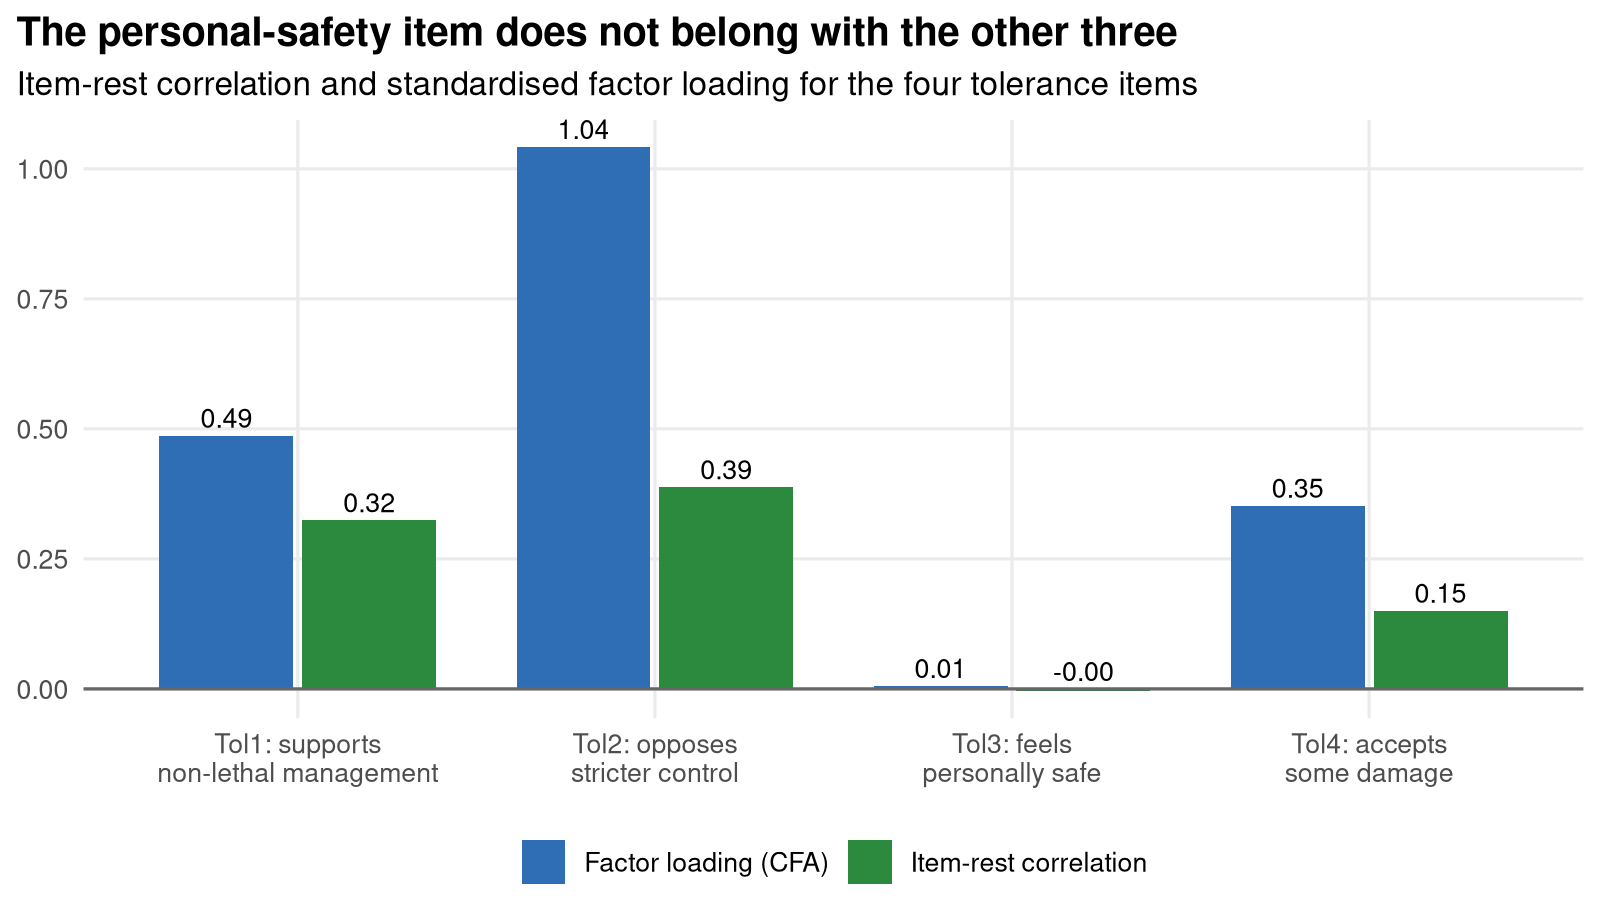
\includegraphics[width=0.85\textwidth]{figures/fig_tol_items.png}
\caption{Item-rest correlation and standardised CFA loading by tolerance
item. Tol3 is indistinguishable from zero on both measures. The Tol2 loading
above 1 is the improper solution discussed in the text.}
\label{fig:tol-items}
\end{figure}

Figure~\ref{fig:tol-items} shows the same pattern graphically: Tol3's bars
are flat on the floor on both measures, while the other three items are
clearly elevated. On this basis we defined the primary tolerance
construct as the three-item composite Tol1+Tol2+Tol4, and kept the original
four-item version only as a named robustness variant. Dropping Tol3 raises
reliability from $\alpha = 0.34$ to $\alpha = 0.50$ (ordinal $\alpha = 0.62$,
computed from polychoric rather than Pearson item correlations, which better
suit five-category ordinal data); every downstream structural path reported
in Section~\ref{model} is materially unchanged between the three-item and
four-item specifications. We also computed the reliability and validity
statistics that a reflective PLS-SEM construct is usually expected to report:
for the three-item tolerance scale, composite reliability is 0.781 and
average variance extracted (AVE) is 0.551, both above their conventional
0.70 and 0.50 thresholds respectively, even though Cronbach's $\alpha$
(0.577 as reported by the PLS-SEM software, which standardises the items;
0.50 on the raw items) and $\rho_A$ (0.620) remain below 0.70. This split is expected for a short, unevenly-loading three-item
composite (Tol2 loads far more strongly than Tol4) and is a known limitation
of $\alpha$ and $\rho_A$ for such scales, not a contradiction of the CFA
result above. Figure~\ref{fig:reliability} shows the progression from the
original four-item raw alpha through the two three-item variants, alongside
the conventional 0.70 threshold.

\begin{figure}[htbp]
\centering
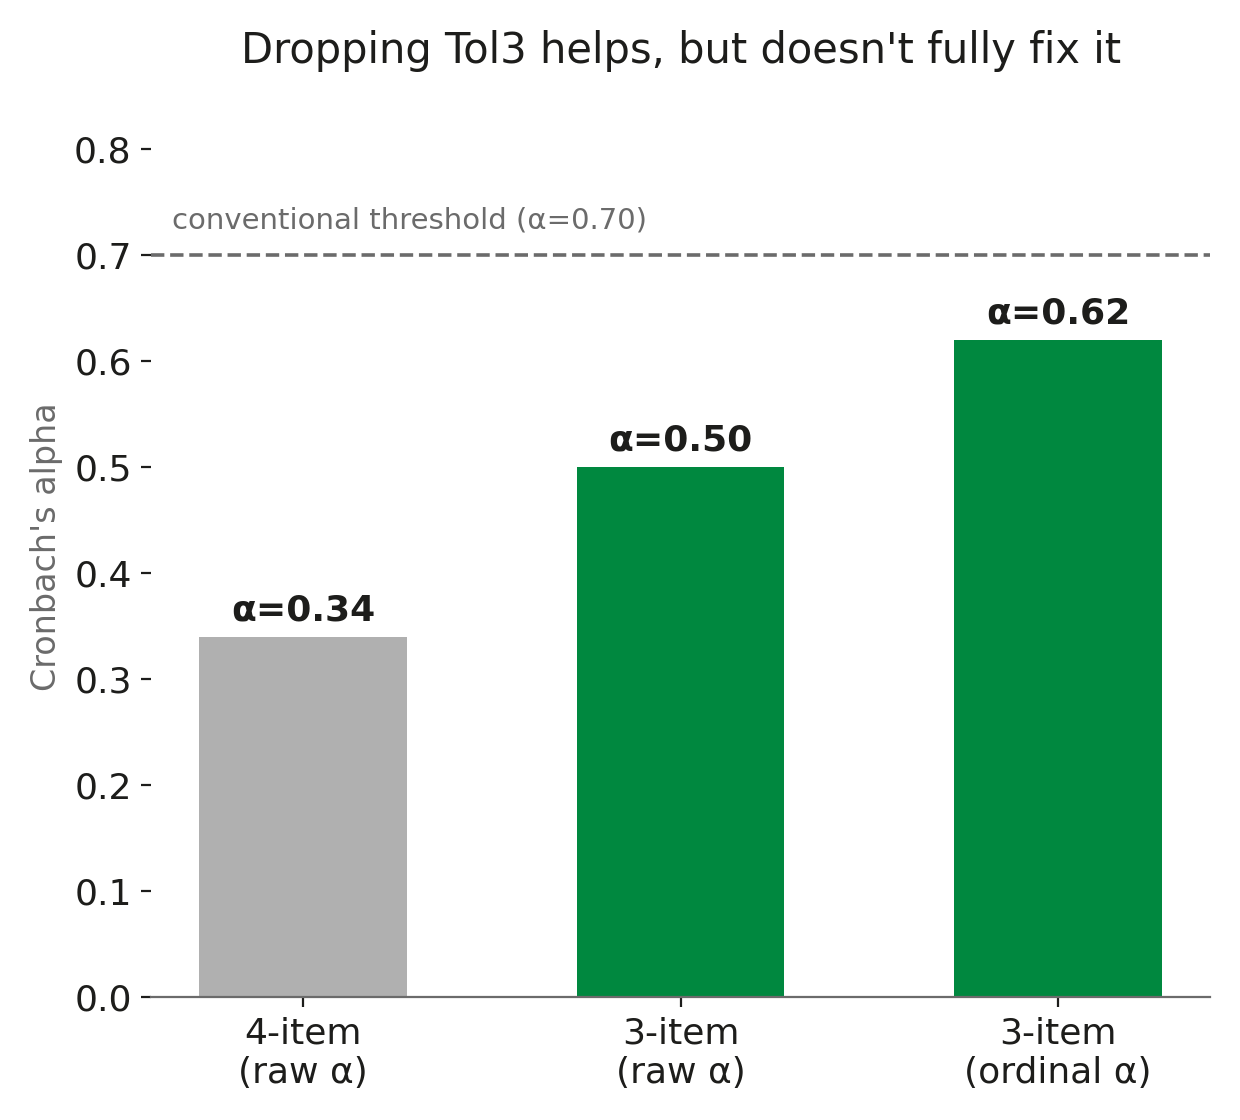
\includegraphics[width=0.75\textwidth]{figures/fig_reliability.png}
\caption{Tolerance scale reliability (Cronbach's $\alpha$): four-item raw,
three-item raw, and three-item ordinal (polychoric), against the
conventional 0.70 threshold.}
\label{fig:reliability}
\end{figure}

\subsection{Formative versus reflective: intangible cost}
\label{measurement:formative}

A second measurement question concerns how intangible cost (IC) -- a
respondent's general evaluative attitude toward wild boar, together with a
spontaneous emotional reaction captured in a three-word description -- should
be modelled: as a \emph{reflective} construct, whose indicators are
interchangeable symptoms of one underlying attitude (as tolerance is treated
above), or as a \emph{formative} construct, whose indicators are distinct
ingredients that combine to define the construct, and need not correlate with
each other at all.

The original questionnaire design specifies intangible cost, alongside
conflict experience, tangible cost, compensation anticipation, and policy
support, as formative by default. We tested this assumption in two ways.
First, EFA on intangible cost's own items shows weak-to-absent common-factor
structure (KMO $= 0.51$; parallel analysis suggests essentially zero
underlying factors) -- the items do not behave like correlated symptoms of one
hidden cause, which is expected and unproblematic for a formative composite,
but would be a problem if IC were meant to be reflective. Second, and more
directly, we forced intangible cost into a reflective specification and
tested its discriminant validity against tolerance using the
heterotrait-monotrait ratio of correlations (HTMT; \citealp{Henseler2015}).
For this test the reflective intangible-cost factor used its two complete
items, the general attitude rating and the first word rating; the second
and third word ratings were left out because many respondents gave fewer
than three words. The result was HTMT $= 1.17$, above the conventional 1.0 ceiling: under a
reflective assumption, the model cannot statistically distinguish intangible
cost's items from tolerance's items at all. This second, more aggressive test
was reserved for intangible cost specifically -- rather than for tangible
cost or the other formative constructs -- because IC's items are the ones
conceptually closest to tolerance itself (an attitude and an emotional
reaction, rather than a physical damage measure), making it the one construct
where a measurement-model mistake could plausibly conflate a predictor with
the outcome it predicts.

Taken together, both checks point the same way: intangible cost is retained
as a formative composite, as originally specified. Its indicators are
ingredients that build the concept, not interchangeable symptoms of it, and
treating it as reflective would have been the wrong measurement choice --
not merely a weaker one.

\subsection{Why tolerance is reflective and intangible cost is formative}
\label{measurement:why-different}

Treating one construct as reflective and another as formative is not an
inconsistency: the choice is made construct by construct, and it is a
conceptual decision about the direction of the relationship between a
construct and its items, not a statistical one. The standard criteria
\citep{Jarvis2003} ask four questions. Does the construct cause the item
responses (reflective), or do the items together make up the construct
(formative)? Are the items interchangeable? Should they correlate with
each other? And does dropping an item change what the construct means?

For tolerance, the Wildlife Tolerance Model \citep{Kansky2016} treats the
items as expressions of one underlying disposition: a more tolerant resident
is expected to support non-lethal management, oppose stricter control, and
accept some damage, all at once. That is the reflective logic, and it is why
we could test it with factor analysis and drop Tol3 without redefining the
construct. For intangible cost, the items are a general attitude rating and
the valence of up to three freely chosen words. The original model specifies
this block, like the other cost and experience blocks, as an index built
from its components, which need not correlate.

We do not want to overstate how clean this distinction is. The empirical
checks are compatible with our choice but do not prove it. Tolerance's
reliability is modest even after dropping Tol3
(Section~\ref{measurement:efa-cfa}), and its three items cover different
content, so a formative reading of tolerance is defensible too. Conversely,
an attitude rating and word valences could reasonably be read as expressions of
one attitude, that is, as reflective. Weak correlations among items do not by themselves make a
construct formative. For this reason we checked whether the choice matters.
Re-estimating the full model with tolerance weighted formatively (PLS mode~B)
instead of reflectively (mode~A) leaves the results unchanged: the
compensation path is $-0.108$ instead of $-0.109$, intangible cost $-0.334$
instead of $-0.338$, intangible benefit $+0.162$ instead of $+0.156$,
prevention effectiveness $+0.107$ instead of $+0.113$, all still
significant, and $R^2$ is $0.235$ instead of $0.234$. The alternative
for intangible cost was tested in Section~\ref{measurement:formative}: as a
reflective construct it cannot be separated from tolerance. Our conclusions
therefore do not depend on the reflective/formative labels, but the closeness
of intangible cost to tolerance is a limitation in either specification
(Section~\ref{discussion:limitations}).

\subsection{Feature engineering}
\label{measurement:features}

Three engineered features feed into the main model. First, as described
above, tolerance enters as the three-item composite Tol1+Tol2+Tol4. Second,
all skewed monetary and area variables (household income, household assets,
economic loss from damage, insurance willingness-to-pay, damaged crop area)
are log(1+x)-transformed. Third, survey site (Baoxing vs.\ Qingchuan) is
engineered as an explicit binary covariate, because Section~\ref{data:confound}
showed that compensation participation is strongly confounded with county;
without this covariate, county differences would be invisible to the model
and could be misattributed to compensation status or conflict experience.

We additionally engineered, but did not use as a control in the primary
model, a household wealth/livelihood index via principal component analysis
(PCA; R package \texttt{factoextra} \citep{Rfactoextra}) on 15 previously-unused variables (crop areas by type, livestock counts
by type, and total land/livestock/asset value). The first principal component
explains 27.9\% of the variance in these 15 variables and correlates strongly
with total household assets ($r = 0.75$) but only weakly with annual cash
income ($r = 0.17$), indicating that income is a poor proxy for asset wealth
in this sample. This index does not predict tolerance directly ($p = .33$),
but it does predict self-reported economic loss strongly
(unstandardised coefficient $0.28$ on log loss, $p < .001$): wealthier households have more agricultural
assets at risk and report more loss accordingly. The original Wildlife
Tolerance Model used a single manifest item (crop asset value) as its only
wealth control; this index shows that a richer, PCA-based wealth measure is
available, though it functions as a socioeconomic control rather than a new
psychological construct, and was therefore not added to the primary
structural model reported in Section~\ref{model}.

\newpage

\section{Main Model and Findings}
\label{model}
\subsection{Why partial least squares structural equation modelling}
\label{model:why-plssem}

We use partial least squares structural equation modelling (PLS-SEM,
R package \texttt{seminr} \citep{Rseminr}) to estimate the full structural model in one
step. PLS-SEM was chosen for three reasons specific to this data. First, it
accommodates formative and reflective constructs simultaneously within a
single estimation: tolerance is reflective (Section~\ref{measurement:tolerance}),
while conflict experience, tangible cost, intangible cost, compensation
anticipation, and policy support are formative
(Section~\ref{measurement:formative}). Second, it does not require
multivariate normality, which is convenient given the skewed monetary
variables described in Section~\ref{data:quality}. Third, it remains reliable
at our sample size ($n = 625$) with a comparatively complex construct
structure.

\subsection{Model specification}
\label{model:spec}

The structural model links four layers of constructs: a background layer
(conflict experience with wild boar and with all species, survey site,
national-park residence, and sociodemographics -- gender, age, education,
income, household assets); an exposure layer (prevention effectiveness and
compensation participation, CE0); a mediator layer (compensation
anticipation, policy support, tangible cost, intangible cost, and intangible
benefit); and the outcome, tolerance. Every construct in an earlier layer has
a direct structural path to every construct in a later layer, including a
direct path from each background variable to tolerance itself; this dense
specification is what lets us report, for example, that a given
predictor's effect on tolerance is estimated \emph{after} already accounting
for site, national-park residence, and demographics in the same equation,
rather than as a separate, unadjusted comparison. Skewed monetary indicators
enter log-transformed within their formative blocks, exactly as in
Section~\ref{measurement:features}. All paths are estimated jointly and
bootstrapped with 5{,}000 resamples to obtain standard errors and $p$-values
for every path simultaneously. Because the underlying data are
cross-sectional and observational, every coefficient below should be read as
an \emph{association}, adjusted for the other variables in the same model,
not as a causal effect.

\subsection{RQ1: does compensation predict tolerance, and is the effect mediated?}
\label{model:rq1}

The full model explains a meaningful share of the variance in tolerance
($R^2 = 0.234$), driven predominantly by intangible cost and, to a lesser
extent, intangible benefit and prevention effectiveness. Table~\ref{tab:rq1}
reports the four direct predictors with a significant path to tolerance.

\begin{table}[htbp]
\centering
\caption{Direct predictors of tolerance with a significant path in the full
structural model ($R^2 = 0.234$; $n = 625$; 5{,}000 bootstrap resamples).}
\label{tab:rq1}
\begin{tabular}{lrr}
\hline
\textbf{Predictor} & \textbf{$\beta$} & \textbf{$p$} \\
\hline
Intangible cost (IC)              & $-0.34$  & $<.001$ \\
Intangible benefit (IB)           & $+0.16$  & $<.001$ \\
Prevention effectiveness (PE)     & $+0.11$  & .005 \\
Compensation participation (CE0)  & $-0.109$ & .003 \\
\hline
\end{tabular}
\end{table}

\begin{figure}[htbp]
\centering
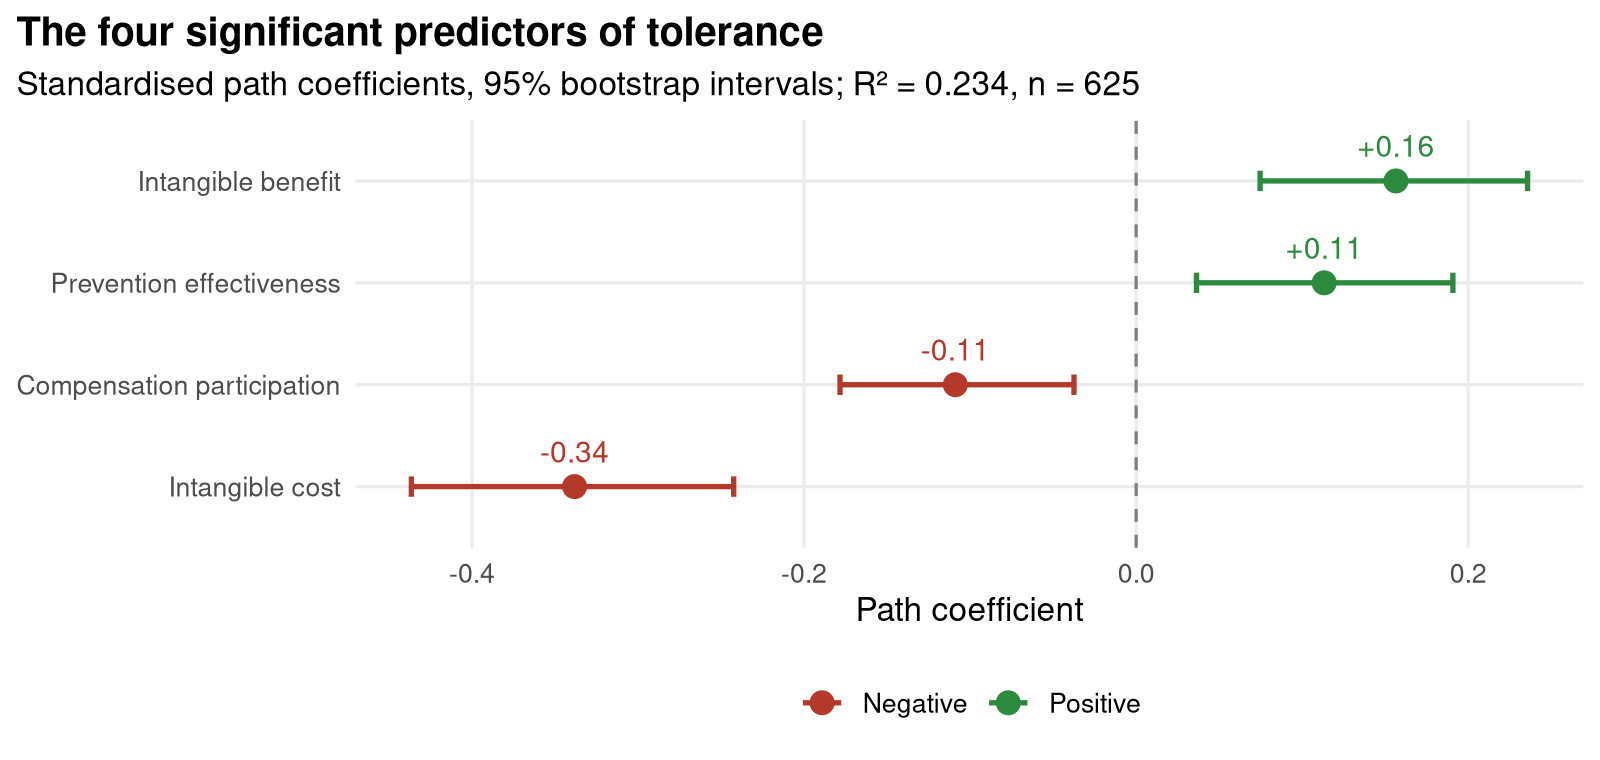
\includegraphics[width=0.8\textwidth]{figures/fig_rq1_paths.png}
\caption{Standardized path coefficients from the four significant direct
predictors of tolerance, with 95\% bootstrap intervals. Red: negative
association; green: positive association.}
\label{fig:rq1-paths}
\end{figure}

\begin{figure}[htbp]
\centering
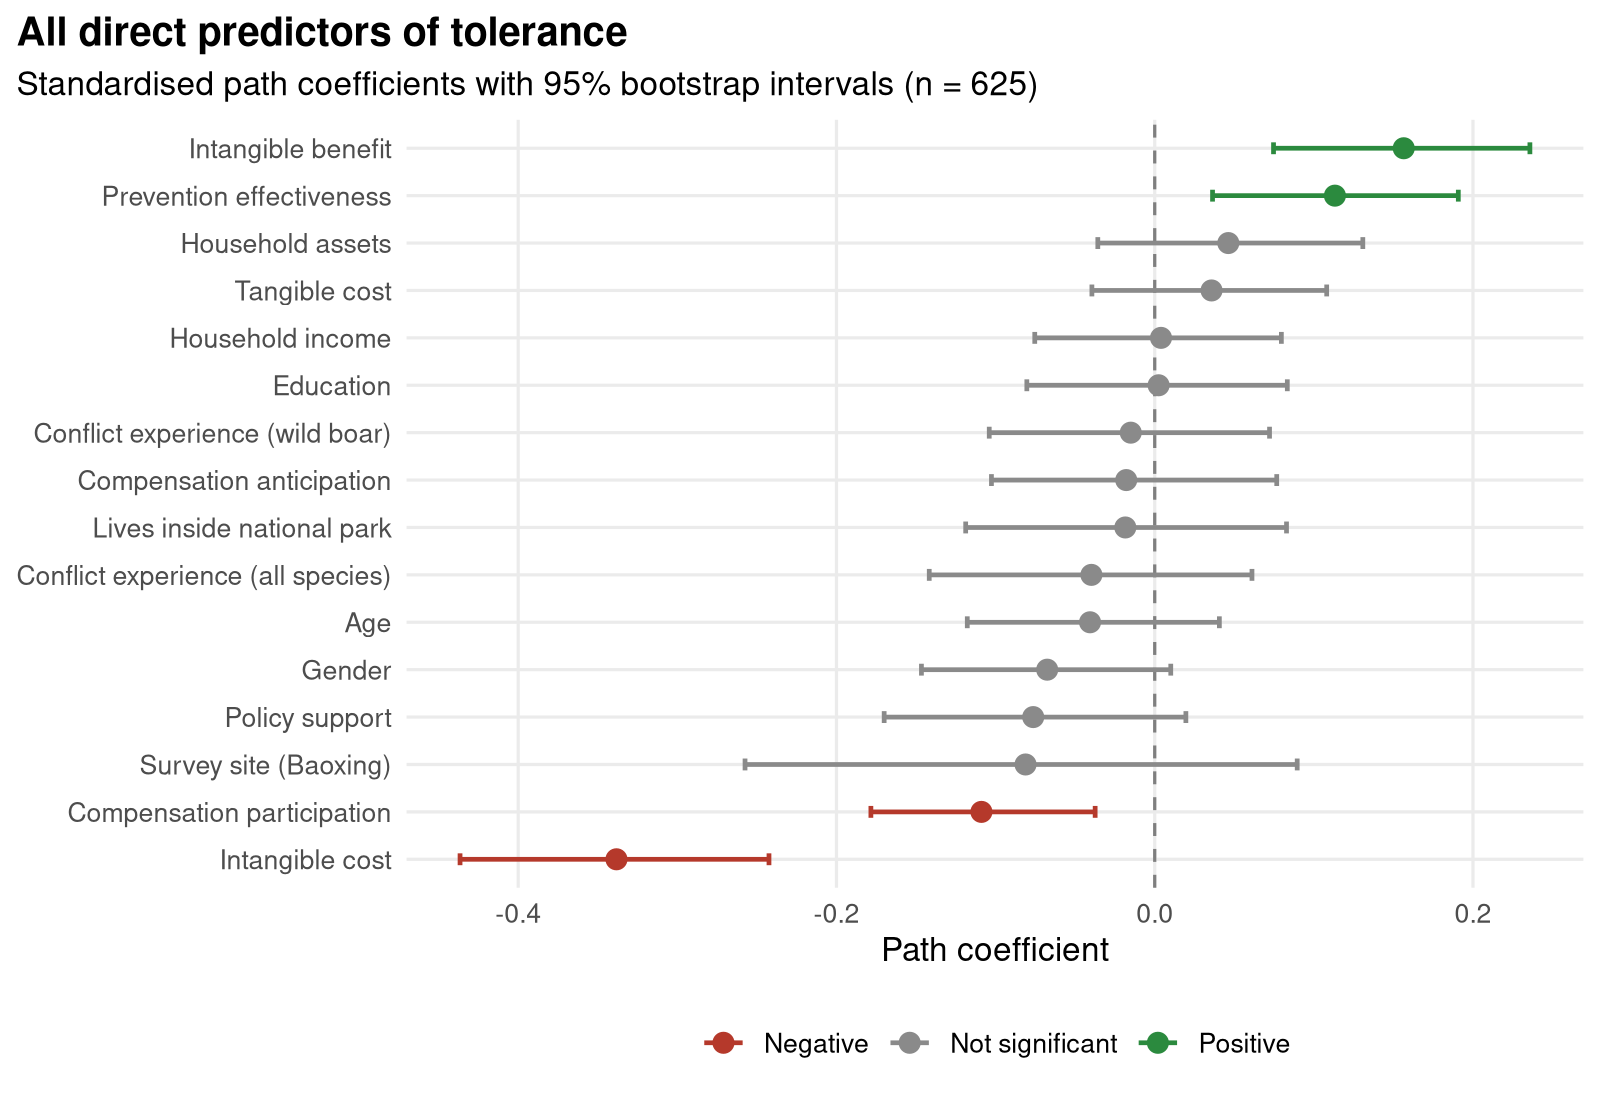
\includegraphics[width=0.85\textwidth]{figures/fig_all_direct_paths.png}
\caption{All direct paths to tolerance in the full structural model, with
95\% bootstrap intervals. Green: positive; red: negative; grey: interval
includes zero.}
\label{fig:all-paths}
\end{figure}

Figure~\ref{fig:rq1-paths} shows all four paths together; Figure~\ref{fig:all-paths}
shows every direct path to tolerance in the model, including those that
are not significant. Intangible cost has the strongest association with tolerance of any
predictor in the model ($\beta = -0.34$, $p < .001$): residents who perceive
more intangible cost from wild boar report markedly lower tolerance.
Intangible benefit ($\beta = +0.16$, $p < .001$) and prevention effectiveness
($\beta = +0.11$, $p = .005$) both associate positively with tolerance.
Compensation participation itself has a smaller, but still significant,
negative association with tolerance ($\beta = -0.109$, $p = .003$), even
after adjusting for survey site -- we refer to this as the
\emph{compensation paradox} throughout this report, since it runs opposite
to the policy assumption that compensation should raise tolerance.

A conceptual point is worth stating clearly before going further, because
the next result can otherwise look like it contradicts the one just given.
Section~\ref{model:rq1} above already established that compensation
participation has a real, statistically robust association with tolerance
(Table~\ref{tab:rq1}; and, as Section~\ref{robustness} shows, that association
is negative in all 8{,}192 alternative model specifications we tested). That
is one question -- \emph{does} compensation participation associate with
tolerance? -- and it has a clear answer: yes. Mediation analysis asks a
second, logically separate question: \emph{through which of our measured
variables} does that association travel? An effect can be real, large, and
completely robust while none of a specific, finite list of candidate
mediators explains it -- this happens whenever the true mechanism runs
through something the study did not measure. Finding no significant
mediator among the five we tested therefore does not weaken or cast doubt on
the direct effect established above; it means only that this particular
analysis cannot yet say \emph{why} the effect exists, which is precisely the
open question this subsection reports.

With that distinction in mind: we tested whether the compensation--tolerance
association runs through the five measured mediator constructs
(compensation anticipation, policy support, tangible cost, intangible cost,
and intangible benefit), using bootstrapped specific-indirect-effect tests
\citep{Nitzl2016}. Table~\ref{tab:mediation} reports the result: none of the
five specific indirect paths is individually significant (all $p > .16$),
and the total indirect effect summed across all five is small ($-0.024$),
corresponding to a variance-accounted-for (VAF) of 18\% of the total
compensation--tolerance association.

\begin{table}[htbp]
\centering
\caption{Bootstrapped specific-indirect-effect tests for compensation
participation $\rightarrow$ mediator $\rightarrow$ tolerance
\citep{Nitzl2016}, with 95\% percentile bootstrap confidence intervals.
Direct effect: $-0.109$ ($p=.003$). Total indirect effect: $-0.024$
(VAF $=18\%$).}
\label{tab:mediation}
\begin{tabular}{llrrrr}
\hline
\textbf{Code} & \textbf{Construct} & \textbf{Indirect effect} & \textbf{SE} & \textbf{95\% CI} & \textbf{$p$} \\
\hline
CA & Compensation anticipation & $-0.0017$ & 0.0046 & $[-0.010,\ 0.009]$ & .800 \\
PS & Policy support            & $-0.0013$ & 0.0054 & $[-0.013,\ 0.010]$ & .808 \\
TC & Tangible cost             & $+0.0027$ & 0.0036 & $[-0.003,\ 0.011]$ & .382 \\
IC & Intangible cost           & $-0.0178$ & 0.0141 & $[-0.048,\ 0.008]$ & .165 \\
IB & Intangible benefit        & $-0.0060$ & 0.0070 & $[-0.021,\ 0.007]$ & .354 \\
\hline
\end{tabular}
\end{table}

In other words, most
of the compensation paradox is not explained by the mediators we measured.
The confidence intervals show how strong this statement is. A
non-significant indirect effect is an absence of evidence, not evidence of
absence: the interval for intangible cost, the most plausible mediator, runs
from $-0.048$ to $+0.008$, so an indirect path of up to roughly 40\% of the
direct effect remains compatible with the data. With a bootstrap standard
error of 0.014, this design would detect an indirect effect through
intangible cost with 80\% power only if it were about 0.04 or larger. The
other four intervals are much tighter around zero. So this does not mean
there is no mechanism connecting compensation to tolerance. Two explanations
remain open. The mechanism may run through
something outside this measurement model: unmeasured grievance related to the
compensation process, prior conflict history not captured by our conflict-
experience items, or some other shared cause behind both compensation-seeking
and lower tolerance. Alternatively, the mediators may be measured too
noisily to carry the effect they really transmit; we examine this second
possibility in Section~\ref{discussion:sensitivity}. This is an open question for future data collection
(Section~\ref{discussion}), not a settled mechanism.

Why do the cost constructs, which the Wildlife Tolerance Model places between
compensation and tolerance, not act as mediators here? An indirect effect is
the product of two legs: compensation must predict the mediator, and the
mediator must predict tolerance. Figure~\ref{fig:mediation-legs} shows both
legs for each construct. Intangible cost and intangible benefit clearly
predict tolerance (second leg), but compensation participation does not
predict either of them once county, conflict experience, and demographics
are adjusted for (first leg: $+0.05$ and $-0.04$, both intervals include zero).
Tangible cost fails on both legs: applicants report somewhat more damage
($+0.07$, not significant), and damage is unrelated to tolerance ($+0.04$).
In plain terms, applicants and non-applicants perceive similar costs and
benefits of wild boar, so those perceptions cannot be what makes applicants
less tolerant. The same logic explains the absence of moderation in
Section~\ref{model:rq2}: costs and benefits relate to tolerance in the same
way in both groups.

\begin{figure}[htbp]
\centering
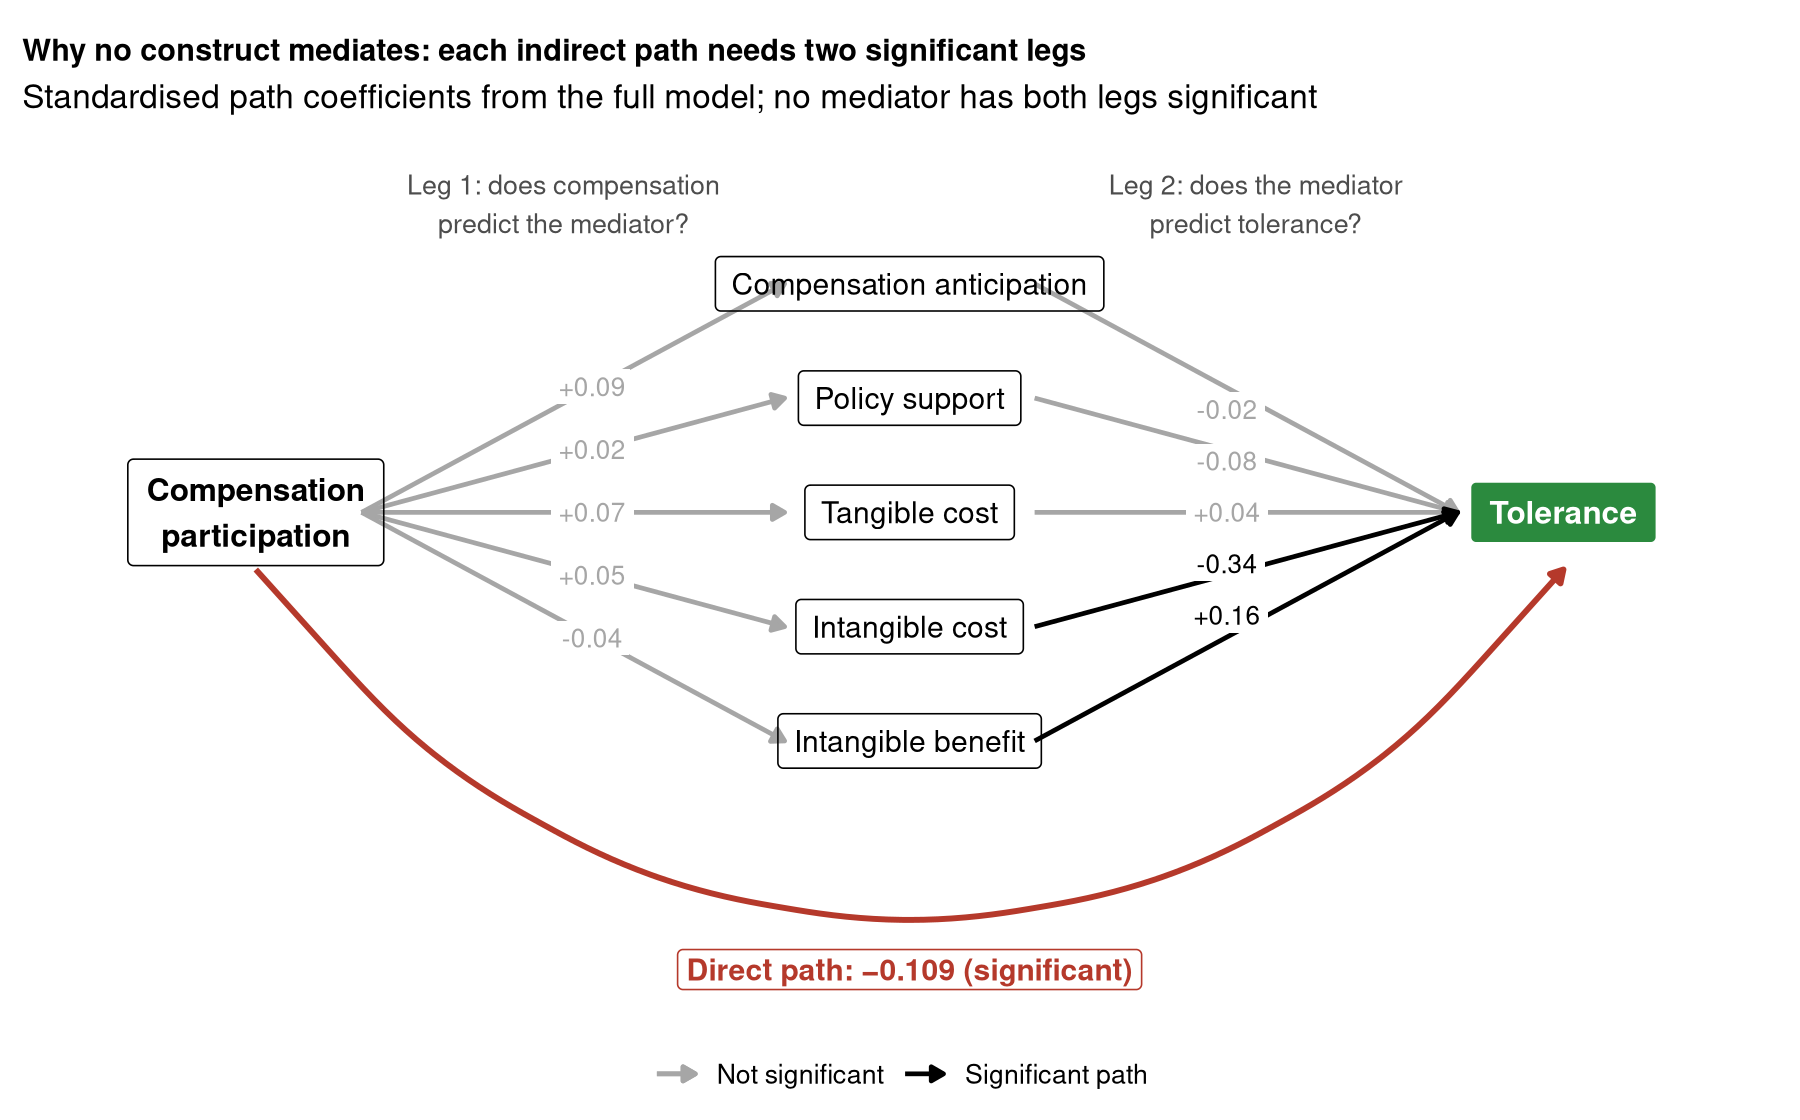
\includegraphics[width=0.95\textwidth]{figures/fig_mediation_legs.png}
\caption{The two legs of each indirect path from compensation participation
to tolerance. Black arrows: 95\% bootstrap interval excludes zero; grey:
includes zero. No construct has two black legs.}
\label{fig:mediation-legs}
\end{figure}

\begin{figure}[htbp]
\centering
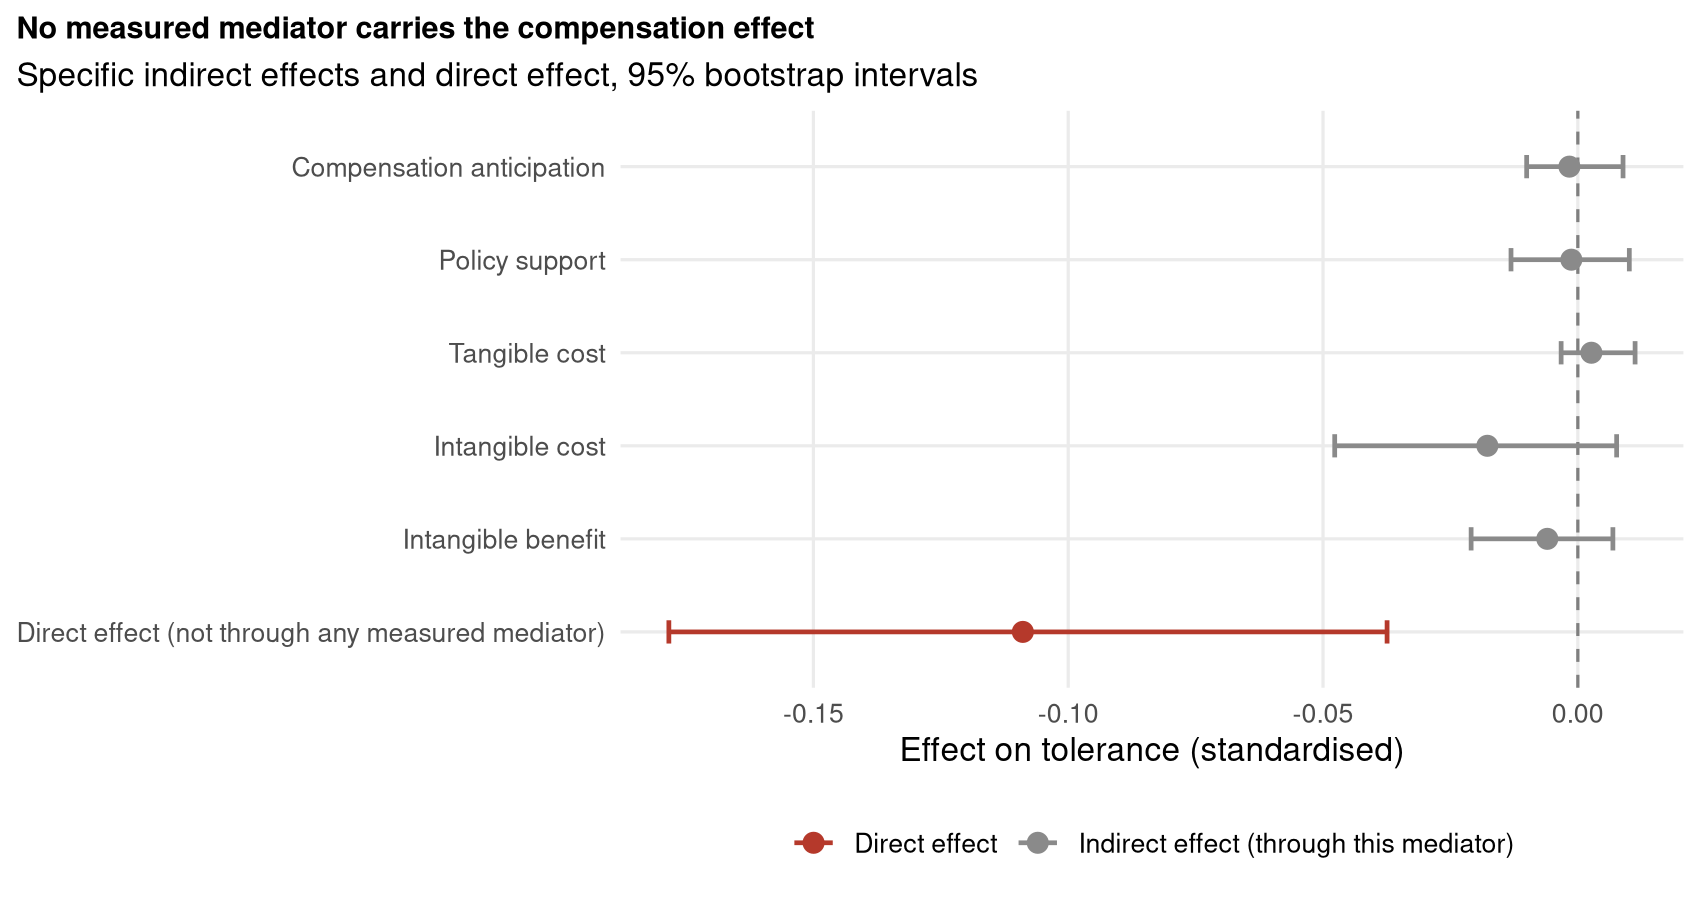
\includegraphics[width=0.9\textwidth]{figures/fig_mediation.png}
\caption{Specific indirect effects of compensation participation on
tolerance (grey) and the direct effect (red), with 95\% bootstrap intervals.
All five indirect intervals include zero; the direct effect does not.}
\label{fig:mediation}
\end{figure}

\subsection{Model checks on individual paths}
\label{model:checks}

Three additional checks qualify how confidently individual paths above
should be read. First, as already noted in Section~\ref{measurement:tolerance},
tolerance's reliability, while improved by dropping Tol3, still falls short
of the conventional threshold by the $\alpha$ and $\rho_A$ criteria; treat
tolerance throughout as a meaningful but noisy measure. Second, policy
support overlaps empirically with conflict experience and with survey site:
HTMT is 1.01 against conflict experience and 1.22 against site, both above
the 1.0 ceiling that normally signals a discriminant-validity problem. The two conflict-experience constructs also overlap with each other (HTMT
1.17). HTMT was designed for reflective constructs, and here it is applied to
formative composites and single items, so these values are a warning sign
rather than a formal test. We
therefore do not build a strong substantive claim on the policy-support path
in isolation -- whatever that path's coefficient captures may be entangled
with conflict experience and site rather than policy support specifically.
Third, survey site significantly predicts all five mediator constructs
(policy support, tangible cost, intangible cost, and intangible benefit at
$p < .001$; compensation anticipation at $p = .044$), but has no significant
remaining direct path to tolerance once those mediators are in the model
($\beta = -0.08$, $p = .34$). We read this as reassuring rather than
concerning: site's entire detectable influence on tolerance appears to run
through the mediators already in the model, rather than through some
separate, unmodelled channel.

\subsection{RQ2: do costs and benefits work differently after compensation?}
\label{model:rq2}

RQ2 asks whether the relationships between costs/benefits and tolerance
change depending on compensation experience -- that is, whether compensation
\emph{moderates} these relationships. We tested this directly with three
interaction terms (compensation participation $\times$ tangible cost,
$\times$ intangible cost, and $\times$ intangible benefit) in a two-stage
moderation model, rather than by comparing separately-fitted coefficients in
each group. The interaction-term approach is the stronger test: comparing two
separately-estimated group coefficients only tells you the two numbers look
different, not whether that difference is statistically distinguishable from
sampling noise in two smaller subsamples; a formal interaction term tests the
difference in slopes directly, using the full sample in one joint estimation.

All three interactions are non-significant (tangible cost $\times$
compensation, $p = .216$; intangible cost $\times$ compensation, $p = .234$;
intangible benefit $\times$ compensation, $p = .899$). This first moderation
model contains only the three cost and benefit constructs, compensation
participation, and their interactions. Because compensation participation is
confounded with county (Section~\ref{data:confound}), we repeated the test
with the full control set of the main model in the tolerance equation
(survey site, national-park residence, both conflict-experience constructs,
demographics, prevention effectiveness, compensation anticipation, and policy
support). The conclusion is the same: $p = .312$, $.142$, and $.871$
respectively, with compensation participation itself still negative
($\beta = -0.106$, $p = .004$). An ordinary regression on observed scores
with the same controls agrees, both for the single interactions (all
$p > .31$) and for a joint test of all three ($F = 0.49$, $p = .69$). The cost/benefit
relationships with tolerance are the same strength regardless of
compensation status: intangible cost remains the strongest negative
predictor and intangible benefit remains positive in both groups, and
compensation experience does not alter either slope. Figure~\ref{fig:interaction-forest} plots the three interaction coefficients
with their intervals, for the model without and with controls: all include
zero. One exploratory observation qualifies this. If interactions of the
costs and benefits with \emph{county} are added to the observed-score
regression as well, the intangible cost $\times$ compensation term
($+0.21$, $p = .028$) and the intangible cost $\times$ county term ($-0.26$,
$p = .029$) both become nominally significant, with opposite signs. These
are two of six additional tests, they are not corrected for multiplicity, and
compensation and county are too entangled to separate cleanly in this way, so we
report it only as an indication that the strength of the intangible
cost--tolerance relationship may vary across settings, not as a finding. Figure~\ref{fig:slopes} shows the
same question informally, as fitted lines of tolerance against each predictor
separately for applicants and non-applicants. These raw lines are
unadjusted, so differences in their slopes (for instance for intangible
benefit) can reflect other differences between the groups; the adjusted
interaction tests in Figure~\ref{fig:interaction-forest} are the
formal answer.

\begin{figure}[htbp]
\centering
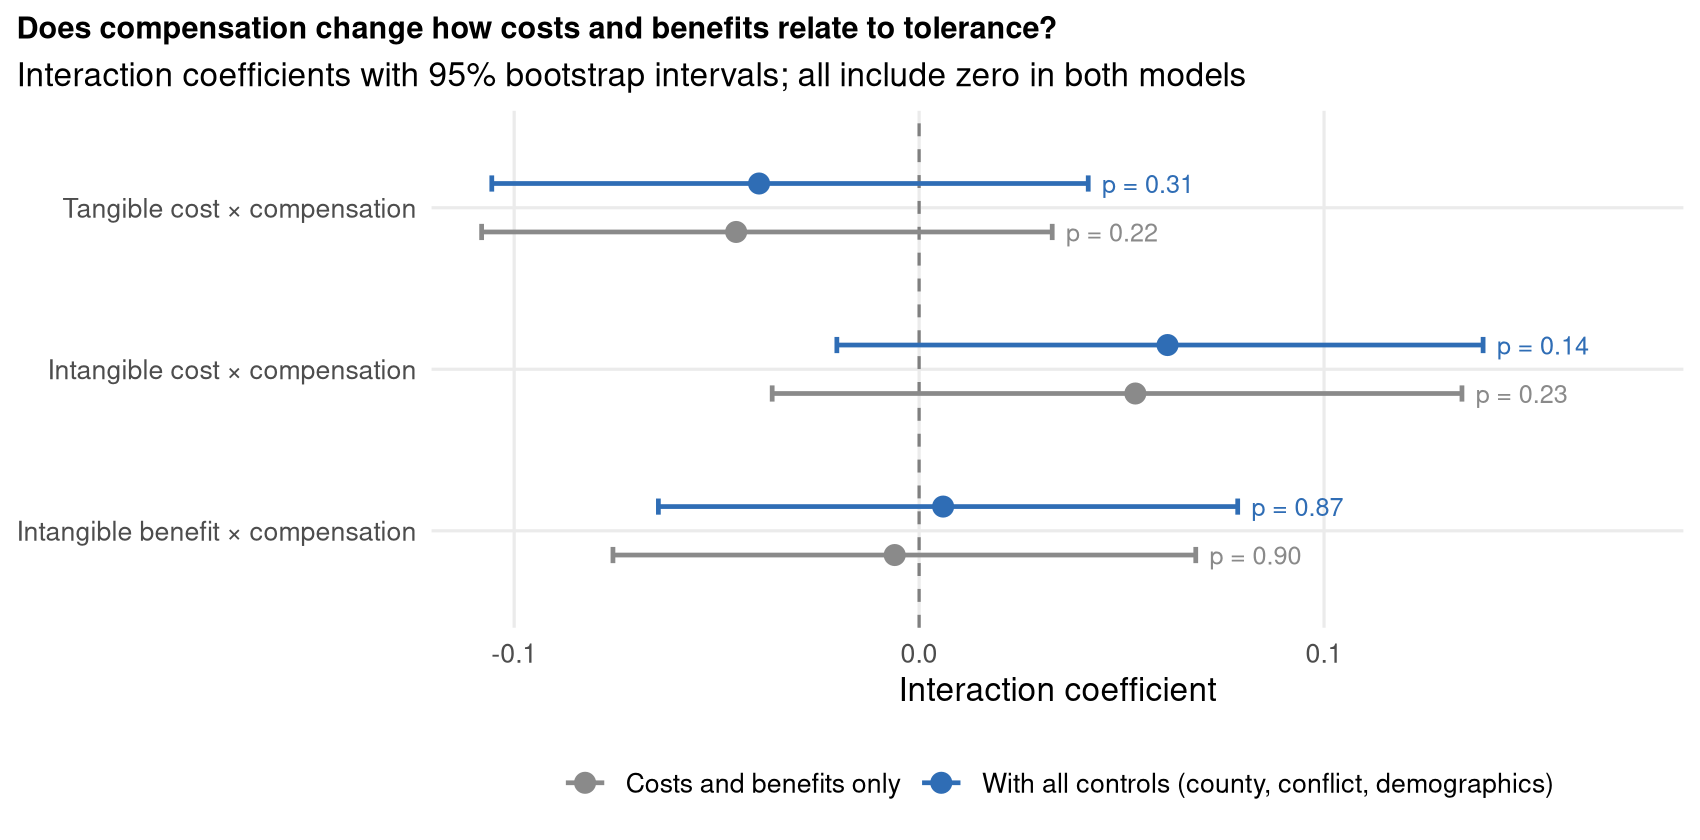
\includegraphics[width=0.9\textwidth]{figures/fig_interaction_forest.png}
\caption{Interaction coefficients (compensation participation $\times$
cost or benefit) on tolerance, with 95\% bootstrap intervals, from the
model with costs and benefits only (grey) and the model with the full
control set (blue).}
\label{fig:interaction-forest}
\end{figure}

\begin{figure}[htbp]
\centering
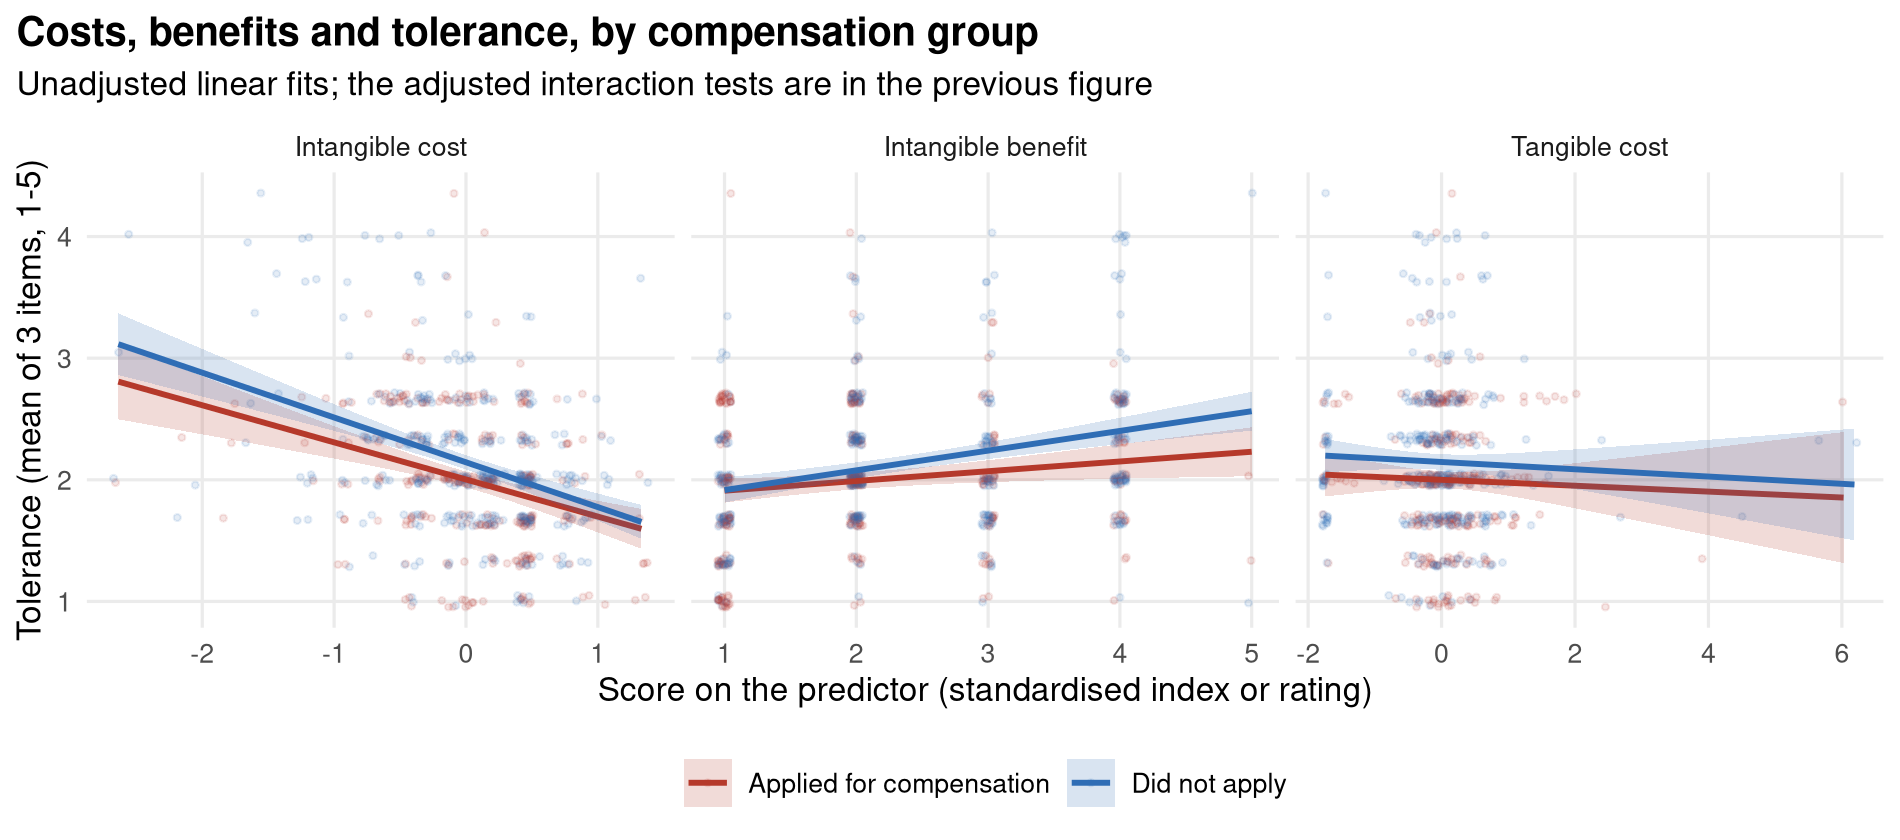
\includegraphics[width=\textwidth]{figures/fig_slopes_by_group.png}
\caption{Tolerance against intangible cost, intangible benefit, and
tangible cost, separately for households that did and did not apply for
compensation (unadjusted linear fits with 95\% confidence bands).}
\label{fig:slopes}
\end{figure}

\subsection{Summary of the main-analysis findings}
\label{model:summary}

For RQ1, compensation participation is negatively associated with tolerance,
and no specific measured mediator explains why. For RQ2, intangible cost is
the strongest negative predictor of tolerance and intangible benefit is a
positive one, and compensation status does not change the strength of
either relationship. Both findings are associations from a single
cross-sectional survey with an incomplete measurement model; they motivate
specific follow-up questions (Section~\ref{discussion}) rather than closing
the topic.

Table~\ref{tab:findings-count} counts what was and was not significant. The
original survey sheet has 57 columns. After removing the identifier, the
township and village labels, the four tolerance items (the outcome), and
the two applicant-only follow-up items, 48 variables remain as candidate
covariates (county enters as survey site). Screened one at a time
(Appendix~\ref{app:screen}), 15 are associated with tolerance at $p < .05$ and
10 after controlling the false discovery rate at 5\%; with county as an
additional covariate, 12 survive. These counts overstate the number of
independent findings, since five of the significant variables are
different indicators of the same construct (intangible cost) and several others
measure conflict with other species. In the full structural model, where the
variables are grouped into constructs and adjusted for each other, four
constructs are significantly associated with tolerance.

\begin{table}[htbp]
\centering
\caption{Summary of significant findings.}
\label{tab:findings-count}
\begin{tabular}{p{4.6cm}p{2.2cm}p{6.2cm}}
\hline
\textbf{Question} & \textbf{Count} & \textbf{Which} \\
\hline
Survey variables associated with tolerance, one at a time (of 48) & 15 nominal; 10 after FDR control & General attitude to wild boar and word ratings (intangible cost), ecological value (intangible benefit), prevention effectiveness, lowest accepted compensation, severity and duration of conflict with all species, potato area \\
Constructs with a significant direct path to tolerance (of 16) & 4 & Intangible cost ($-0.34$), intangible benefit ($+0.16$), prevention effectiveness ($+0.11$), compensation participation ($-0.109$) \\
Significant mediators of the compensation effect (of 5) & 0 & None; total indirect effect $-0.024$ (18\%) \\
Significant interactions with compensation (of 3) & 0 & None, without or with the full control set \\
Significant moderators & 0 in the interaction tests & Compensation status does not moderate any cost or benefit path; the multi-group analysis finds one exploratory difference (Section~\ref{robustness:mga}) \\
\hline
\end{tabular}
\end{table}

\newpage

\section{Robustness and Multi-Group Analysis}
\label{robustness}
RQ3 asks how robust the RQ1/RQ2 findings are to reasonable alternative
analytical choices, and whether they hold across compensation groups. We
address this with two independent exercises: a specification-vibration
analysis across many plausible model variants, and a permutation-based
multi-group analysis (MGA) comparing compensated and uncompensated
residents directly. As the StaBLab consulting-methodology notes that guided
this project put it, the goal of a robustness exercise is not to search for
significant results, but to examine how sensitive the main findings are to
different reasonable analytical choices -- trying many specifications and
reporting only the one that happens to be significant would be a form of
selective reporting, not robustness testing.

\subsection{Specification vibration}
\label{robustness:vibration}

We first compared six theoretically motivated model specifications, each
changing exactly one analytical choice at a time (e.g.\ three-item vs.\
four-item tolerance, alternative cost definitions, alternative control sets).
We then went further and estimated every possible combination of 13 binary
adjustment choices -- $2^{13} = 8{,}192$ models in total -- following the
vibration-of-effects framework of \citet{Patel2015}, who found that
observational associations can flip sign (a "Janus effect") under different,
individually defensible specifications; in their reanalysis of 417
variables, 31\% showed such a sign flip. Across all 8{,}192 model variants
estimated here, the compensation participation -- tolerance association
was negative in every single model (0 Janus effects), and reached
conventional significance ($p < .05$) in 99.4\% of them. The median
standardized coefficient across all 8{,}192 models was $\beta = -0.09$,
consistent with the range obtained across the six theoretically motivated
specifications ($\beta = -0.128$ to $-0.143$) and with the primary model
reported in Section~\ref{model:rq1} ($\beta = -0.109$). We additionally
required every specification to meet minimum measurement-quality bars
(formative outer loadings $\geq 0.70$ where applicable, variance inflation
factor $< 3$) and computed the standardized root mean square residual
(SRMR) across all specifications to confirm that model fit did not degrade
as adjustments were added. On this evidence, the negative
compensation--tolerance association is not an artefact of any single
analytical choice. Appendix~\ref{app:vibration} shows an independent
re-computation of the same exercise on observed (mean-score) variables.

\subsection{Multi-group analysis}
\label{robustness:mga}

The second robustness exercise directly compares the structural model
between the 277 residents with compensation experience (CE0 = 1) and the
348 without (CE0 = 0), using permutation-based multi-group analysis
(1{,}000 permutations). A permutation test makes no distributional
assumption and is appropriate for the two groups' unequal sizes; it tests
whether path coefficients are statistically different across groups, going
beyond an earlier, purely visual sub-group comparison. Before comparing any
path coefficients across groups, we first confirmed that discriminant
validity (HTMT) holds \emph{within} each group separately: an HTMT violation
within a subgroup would make that subgroup's path coefficients unreliable,
and any between-group comparison built on them meaningless. Discriminant
validity held in both groups.

We ran two versions of the comparison: MGA~1, the full model with all
background controls; and MGA~2, with sociodemographic controls removed, as a
confounder check -- if a path difference in MGA~1 disappeared once
demographics were added back and a \emph{different} path emerged once they
were removed, that would suggest the demographics were themselves confounding
the group comparison. In fact, the significant findings in MGA~1 and MGA~2 do
not overlap, and no previously-significant path becomes non-significant when
demographics are added or removed; the confounder check passes.

The core finding, robust across both versions, is one of \emph{structural
invariance}: the model's path coefficients do not differ significantly
between compensated and uncompensated residents for almost every path,
including the intangible-cost -- tolerance path, which is significant in both
groups ($p < .001$ in each). One path is the exception: in MGA~2 (without
demographic controls), conflict experience with all species has a
significantly different relationship with tolerance across the two groups
($\beta = -0.187$ for compensated residents versus $\beta = +0.038$ for
uncompensated residents; $\Delta\beta = -0.225$, $p = .039$). We interpret
this as suggestive evidence that compensation experience may amplify the
conflict--tolerance link: among compensated residents, more conflict
experience associates with markedly lower tolerance, whereas among
uncompensated residents the association is close to zero. We supplemented
the permutation $p$-value, which only tells us whether a difference is
statistically detectable, with Cohen's $f^2$ effect size, which asks how
functionally important each predictor is \emph{within} each group
separately (thresholds: negligible $< 0.02$, small $\geq 0.02$, medium
$\geq 0.15$, large $\geq 0.35$; \citealp{Cohen1988}). In MGA~2, intangible
cost's effect size is medium-to-large among uncompensated residents
($f^2 = 0.258$) and small-to-medium among compensated residents
($f^2 = 0.103$) -- the same pattern of intangible cost mattering more for
uncompensated residents holds across both MGA versions and both ways of
quantifying "matters" (statistical difference and effect size).

Finally, the two groups differ in how much of tolerance the model explains
overall: $R^2 = 0.423$ for uncompensated residents versus $R^2 = 0.299$ for
compensated residents in MGA~1. The model captures uncompensated residents'
tolerance more completely than it captures compensated residents' tolerance.
Read alongside the mediation result in Section~\ref{model:rq1} -- where the
measured mediators account for only 18\% of the compensation--tolerance
association -- this lower $R^2$ points the same direction: compensated
residents' tolerance appears to be shaped by additional factors this model
does not measure, plausibly related to their compensation experience itself
(for example, perceptions of payment adequacy, timeliness, or fairness,
which our questionnaire only captured for a subset of applicants and could
not include in the main structural model; Section~\ref{data:quality}) or to
prior conflict history not captured by our conflict-experience items. This
is precisely the kind of open question a longitudinal or better-instrumented
follow-up study, discussed in Section~\ref{discussion}, would be positioned
to resolve.

To summarize RQ3: the model is structurally stable across compensation
groups on nearly every path, and the negative compensation--tolerance
association from RQ1 does not depend on any single analytical choice among
the 8{,}192 tested. The one genuine group difference we find -- conflict
experience mattering more for compensated residents -- and the lower
explanatory power of the model for that same group, both point toward
unmeasured factors specific to the compensation experience as the most
promising direction for future work.

\newpage

\section{Discussion}
\label{discussion}
\subsection{What our design can and cannot establish}
\label{discussion:design}

Two methodological points are worth stating explicitly, because they define
the boundary of what this analysis can claim.

First, several exhibits in this report -- most notably the covariate-balance
comparison in Section~\ref{data:balance} -- compare the distribution of a
variable (assets, gender, and so on) \emph{conditional on} compensation
group, rather than modelling compensation status as an outcome to be
predicted from those variables. This is a deliberate choice, not an
oversight: its purpose is to check whether the two compensation groups are
comparable before any later comparison is trusted, exactly as a baseline
characteristics table does in an observational or quasi-experimental study.
The complementary, predictive-direction question -- do these same variables
predict who applies for compensation? -- is answered separately, inside the
main structural model itself (Section~\ref{model:spec}), where
sociodemographic and background constructs have explicit paths \emph{to}
compensation participation. There, only household income reaches
significance ($\beta = 0.080$, $p = .047$); gender is borderline
($\beta = 0.069$, $p = .060$); age, education, and household assets are not
significant predictors of compensation participation once the other
background variables are accounted for jointly. Both directions of analysis
appear somewhere in this report; neither substitutes for the other.

Second, every coefficient in this report is an \emph{association}, adjusted
for the other variables in the same model, not a causal effect. The data are
observational and cross-sectional: compensation status was not randomly
assigned, and we do not observe tolerance before a household applied for
compensation. Where we write that compensation participation is "negatively
associated with" tolerance, we mean precisely that and no more.

\subsection{Sensitivity checks on the main finding}
\label{discussion:sensitivity}

We ran three further checks aimed at the most likely ways in which the
compensation paradox could be an artefact. All three are exploratory and
were added after the main analysis; they use ordinary regression on the
construct scores from the main model, or a separate latent-variable model,
and are reported here to qualify the main result, not to replace it.

\paragraph{Does the association hold within each county?} Compensation
status is strongly tied to county (Section~\ref{data:confound}), and with
only two counties a site covariate cannot fully separate the two. We
therefore re-estimated the compensation--tolerance association separately
in each county (Table~\ref{tab:within-county}). The association is negative
in both. In Qingchuan it is clearly different from zero. In Baoxing the
point estimate is, if anything, larger, but the confidence interval is wide
and includes zero: only 41 of the 160 Baoxing respondents did not apply for
compensation, so that comparison is imprecise. A formal
compensation~$\times$~county interaction is not significant ($p = .34$). The
paradox is therefore not produced by pooling two different counties, but the
statistical evidence for it rests mainly on Qingchuan.

\begin{figure}[htbp]
\centering
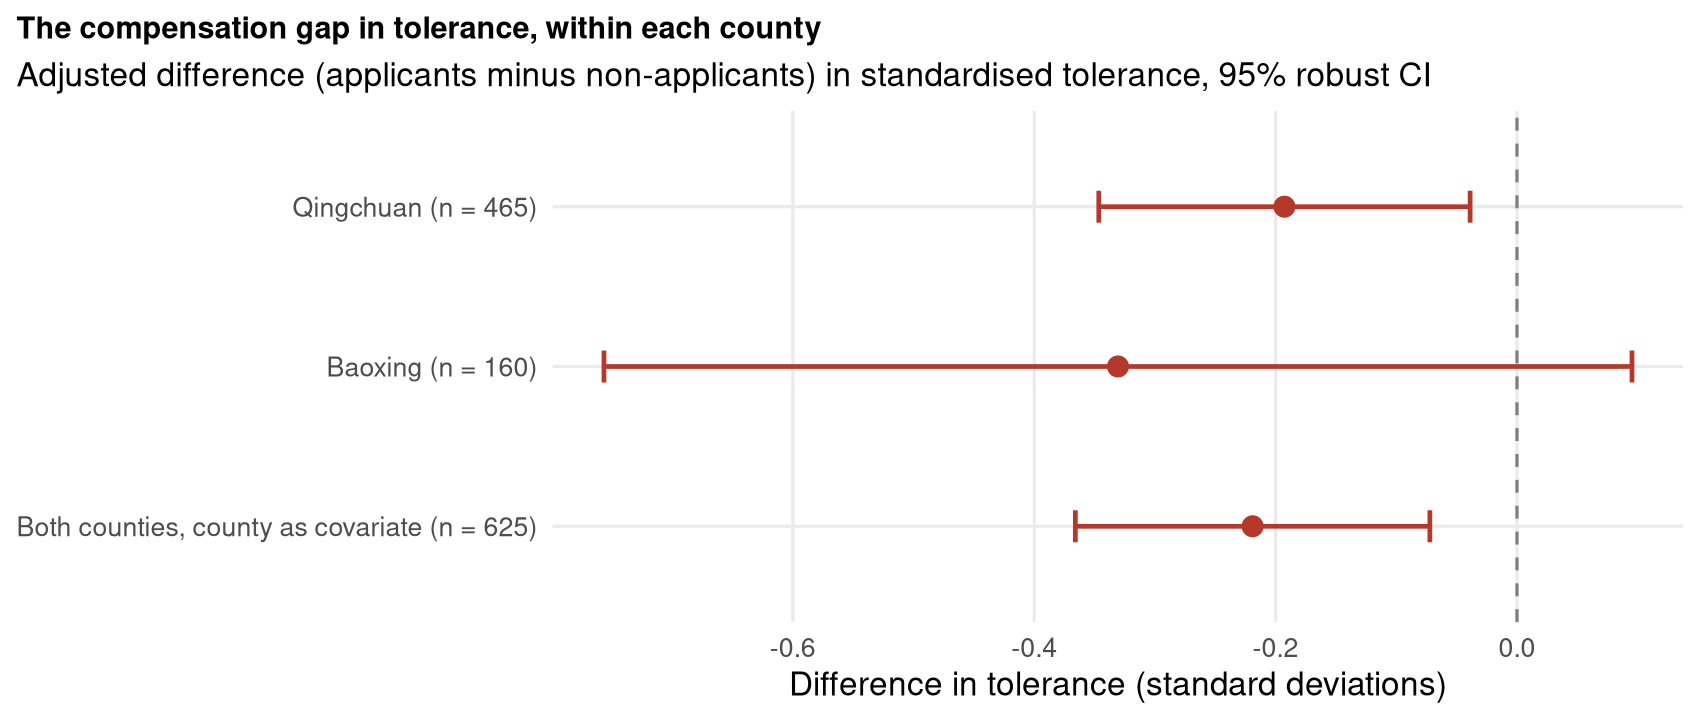
\includegraphics[width=0.9\textwidth]{figures/fig_within_county.png}
\caption{The adjusted compensation gap in tolerance, in each county and with
both counties pooled.}
\label{fig:within-county}
\end{figure}

\begin{table}[htbp]
\centering
\caption{Compensation participation and tolerance within each county.
Entries are the adjusted difference in the standardised tolerance score
between applicants and non-applicants (in standard deviations), from a
linear regression on the construct scores of the main model, controlling
for the background variables and the mediator constructs, with
heteroscedasticity-robust (HC3) standard errors. Because compensation
participation is entered as a 0/1 variable here, these values are on a
different scale from the standardised $\beta$ in Table~\ref{tab:rq1}.}
\label{tab:within-county}
\begin{tabular}{lrrrr}
\hline
\textbf{County} & \textbf{$n$} & \textbf{Difference} & \textbf{95\% CI} & \textbf{$p$} \\
\hline
Qingchuan & 465 & $-0.19$ & $[-0.35,\ -0.04]$ & .014 \\
Baoxing   & 160 & $-0.33$ & $[-0.76,\ 0.10]$  & .127 \\
Pooled, with county as covariate & 625 & $-0.22$ & $[-0.37,\ -0.07]$ & .004 \\
\hline
\end{tabular}
\end{table}

\paragraph{Could measurement error hide a mediator?} Our mediators are short
self-report blocks. Random measurement error in a mediator has two known
consequences, which is why it is a natural suspect for ``missing'' mediation.
First, it causes \emph{attenuation bias}: the estimated effect of the
mediator on tolerance (the second leg) is pulled towards zero, and with it
the indirect effect, which is the product of the two legs. Second, it causes
\emph{incomplete adjustment}: because compensation participation is
correlated with the mediator, part of the mediator's true influence is not
absorbed by the noisy measure and shows up instead as a direct effect of
compensation. Together these can make a truly mediated effect look direct.
PLS-SEM composites do not correct for either problem.

As a sensitivity analysis we refitted the model as a latent-variable model
(R package \texttt{lavaan}, WLSMV estimator), with tolerance as an ordinal
latent factor and \emph{all five} mediators entered together, each as a latent
variable measured by its construct score with an assumed reliability between
1.0 (no error) and 0.6 (Table~\ref{tab:latent}). The same reliability was
applied to every mediator because we have no external estimate for each one.
For the formative constructs, whose indicators are not assumed to be
error-free copies of one quantity, this is a sensitivity assumption, not an
estimated property, and the results should be read in that light.

The result is the same at every assumed reliability. Correcting for error
strengthens the second leg for intangible cost considerably (standardised
path $-0.41$ without correction, $-0.65$ at reliability 0.6) and the
indirect effect through intangible cost grows from $-0.021$ to $-0.044$, but
its interval always includes zero. The indirect effects through the other four
mediators stay close to zero, as does the total indirect effect
($-0.032$ to $-0.049$, intervals including zero throughout), and the direct
association between compensation and tolerance stays negative and different from
zero ($-0.146$ to $-0.129$). The limiting factor is the first leg. Random
error in a mediator that serves as an \emph{outcome} of compensation does not
bias that first-leg coefficient; it only widens its interval. Compensation
participation is barely related to intangible cost ($+0.05$ to $+0.07$,
$p \approx .22$) or intangible benefit ($-0.04$ to $-0.05$, $p = .35$), and
no correction for random error can create a relationship that is not there.
The two mediators with a nominally detectable first leg, compensation anticipation
($+0.09$ to $+0.12$, $p \approx .04$) and, borderline, tangible cost, have a
second leg indistinguishable from zero ($-0.03$ and $+0.02$ to $+0.14$).
We conclude that attenuation from random measurement error does not explain
the absence of mediation in this data. Two other kinds of error are not
covered by this analysis and could work in the opposite direction: error that is
shared between intangible cost and tolerance because both are reported by the
same person (which would inflate their second leg, see
Section~\ref{discussion:limitations}), and error that depends on compensation
status itself (differential error), for instance if applicants rate costs
differently because of their dealings with the compensation process.

\begin{table}[htbp]
\centering
\caption{Latent-variable sensitivity analysis for all five mediators:
standardised indirect effects of compensation participation on tolerance
(95\% CI in brackets) under different assumed reliabilities of the mediator
scores. CA: compensation anticipation; PS: policy support; TC: tangible cost;
IC: intangible cost; IB: intangible benefit. Direct is the compensation
$\rightarrow$ tolerance path. Values are comparable across rows, but not in
size with the PLS-SEM coefficients in Table~\ref{tab:rq1}.}
\label{tab:latent}
\small
\begin{tabular}{crrrrrrr}
\hline
\textbf{Rel.} & \textbf{Direct} & \textbf{via CA} & \textbf{via PS} & \textbf{via TC} & \textbf{via IC} & \textbf{via IB} & \textbf{Total indirect} \\
\hline
1.0 & $-0.15$ & $-0.003$ & $-0.002$ & $+0.001$ & $-0.021$ & $-0.008$ & $-0.032\ [-0.075,\ 0.010]$ \\
0.9 & $-0.14$ & $-0.003$ & $-0.002$ & $+0.002$ & $-0.024$ & $-0.009$ & $-0.035\ [-0.083,\ 0.012]$ \\
0.8 & $-0.14$ & $-0.003$ & $-0.002$ & $+0.004$ & $-0.028$ & $-0.009$ & $-0.039\ [-0.094,\ 0.015]$ \\
0.7 & $-0.13$ & $-0.004$ & $-0.002$ & $+0.007$ & $-0.034$ & $-0.010$ & $-0.044\ [-0.108,\ 0.021]$ \\
0.6 & $-0.13$ & $-0.005$ & $-0.002$ & $+0.013$ & $-0.044$ & $-0.011$ & $-0.049\ [-0.129,\ 0.031]$ \\
\hline
\end{tabular}

\smallskip
\footnotesize The 95\% interval of every individual indirect effect includes zero at all
reliabilities; the direct path is significant ($p < .03$) at all reliabilities.
\end{table}

\paragraph{What the robustness analysis does and does not show.} That the
compensation coefficient is negative in all 8{,}192 specifications
(Section~\ref{robustness}) shows that the result does not depend on our
analytic choices. It does not show that the association is causal, or free
of bias: every specification uses the same respondents, the same
self-reported measures, and the same non-random assignment to compensation,
so any bias from those sources is present in all of them.

\subsection{Limitations}
\label{discussion:limitations}

Five limitations bound every conclusion in this report. First, the
comparison is cross-sectional: we lack each respondent's tolerance before
they applied for compensation, and payment timelines are not consistently
established across respondents, so we cannot rule out that some of the
association we attribute to compensation participation reflects
pre-existing differences between residents who chose to apply and those who
did not. Second, county and survey period coincide completely
(Section~\ref{data:confound}), and the sampling frame and any exclusions
applied before we received the data are incompletely documented; we have
controlled for the county/survey-wave confound statistically, but cannot
rule out other, unrecorded differences between the two fieldwork rounds.
Third, several measurement blocks are short and conceptually overlapping
(Section~\ref{measurement:formative}), and the free-text word responses
used for part of the intangible-cost measure have structural missingness;
together these limit how strongly we can claim to have isolated distinct
latent psychological constructs, as opposed to correlated but imperfectly
separated ones. Fourth, tolerance and intangible cost are both attitudes
reported by the same person in the same interview. A respondent who is
generally aggrieved is likely to rate wild boar more negatively and to
report lower tolerance at once, so part of the strong intangible
cost--tolerance association may reflect shared reporting tendencies rather
than one attitude driving the other; the discriminant-validity result in
Section~\ref{measurement:formative} points the same way. The finding that
intangible cost is the strongest correlate of tolerance should be read with
this in mind. Fifth, tolerance itself is measured with limited reliability
(Section~\ref{measurement:efa-cfa}), and the mediation, moderation, and
multi-group analyses involve many tests on one data set. We treat the
compensation--tolerance path as the one confirmatory result; the mediation
and moderation results are mostly null findings, for which the sample gives
limited power (Section~\ref{model:rq1}), and the single multi-group
difference we report should be regarded as exploratory until replicated.

\subsection{Recommendations for the next study}
\label{discussion:next-steps}

Three concrete steps would materially strengthen the next round of analysis
or data collection. First, several fieldwork details should be clarified
directly with the project partner before any further modelling: the exact
routing between applying for and receiving compensation, which sampling
exclusions were applied and why, precise fieldwork dates, the units
underlying the area variables, and the small number of compensation-
percentage responses that exceed 100\% of assessed loss
(Section~\ref{data:quality}). Second, once those clarifications are in hand,
the report should be revised transparently, re-running only the specific
analyses that those clarifications affect, rather than the full pipeline,
so that the provenance of every number remains traceable. Third, and most
importantly for RQ1, a future panel study should measure tolerance and
related attitudes \emph{before} a household applies for compensation and
again \emph{after} payment is received, with a clearer set of indicators and
an explicit comparison design. Only a before/after design of this kind can
distinguish whether compensation genuinely lowers tolerance, whether
lower-tolerance households are simply more likely to apply in the first
place, or whether both are downstream of some third factor -- such as prior
conflict severity or grievance with the compensation process itself -- that
the present cross-sectional survey cannot measure.

\newpage

\section{Conclusion}
\label{conclusion}
This project set out to test whether compensation for wild boar damage
raises tolerance toward wild boar among residents of two counties bordering
Giant Panda National Park, and, if not, why not. Across 625 households, we
find the opposite of the policy assumption: compensation participation is
associated with \emph{lower}, not higher, tolerance ($\beta = -0.109$,
$p = .003$), even after adjusting for the strong confound between
compensation status and county of residence ($\chi^2 = 77.1$, $p < .001$).
This compensation paradox is not explained by the five mediating constructs
we measured -- compensation anticipation, policy support, tangible cost,
intangible cost, and intangible benefit account for only 18\% of the total
association (RQ1) -- and it does not depend on how costs and benefits
interact with compensation status, since none of the three tested
interaction terms is significant (RQ2). The paradox also survives extensive
robustness testing: it is negative in all 8{,}192 alternative model
specifications we estimated, and the underlying structural model is largely
invariant between compensated and uncompensated residents, with one
exception -- conflict experience with wildlife more broadly matters more for
compensated residents' tolerance than for uncompensated residents' (RQ3).

Throughout, intangible cost -- residents' general evaluative attitude and
emotional reaction toward wild boar -- is the strongest single predictor of
tolerance in every specification and every subgroup we tested, consistently
outweighing compensation status itself. This points toward a broader
conclusion than a narrow one about compensation policy: efforts to improve
tolerance that focus only on offsetting tangible economic loss are targeting
a secondary driver. The primary driver, in this data, is how residents feel
about wild boar and their own capacity to cope with living alongside them --
dimensions that a compensation payment alone does not address.

Two things follow for how these results should be used. First, they should
be read as a robust, well-tested \emph{association}, not as evidence that
compensation payments themselves cause lower tolerance; the cross-sectional
design cannot rule out that residents who were already less tolerant were
also more likely to apply. Second, resolving that ambiguity -- and
identifying what, beyond the five mediators tested here, actually connects
compensation experience to tolerance -- is squarely a question for the
longitudinal, before/after study design recommended in
Section~\ref{discussion:next-steps}, not for further re-analysis of the
present cross-sectional data.


\newpage

% ------------------------------------------------------------------------------
% CONTRIBUTIONS ------------------------------------------------------------------
% ------------------------------------------------------------------------------

\section*{Contributions}
\addcontentsline{toc}{section}{Contributions}
\label{contributions}
This report and the underlying analysis were produced collaboratively by the
three authors, alongside project partner Mengxi Kou and supervisors
Dr.\ Sabine Hoffmann and Marie Scherzer. Primary responsibility for each part
of the analysis, the presentation, and this report was divided as follows.

\begin{itemize}
  \item \textbf{Vaishali Iyer:} \textcolor{orange}{[to be completed --
    e.g.\ which sections of the data preparation, exploratory analysis, or
    report she led]}
  \item \textbf{Jihao Li:} \textcolor{orange}{[to be completed -- e.g.\
    which sections of the data preparation, exploratory analysis, or report
    he led]}
  \item \textbf{Duc-Anh Nguyen:} led the measurement-model refinement
    (Section~\ref{measurement}), the primary structural (PLS-SEM) model and
    the RQ1/RQ2 findings (Section~\ref{model}), the specification-vibration
    and permutation-based multi-group robustness analysis
    (Section~\ref{robustness}), and drafted this report.
\end{itemize}

All three authors reviewed and approved the final presentation and this
report.

\newpage

% ------------------------------------------------------------------------------
% LIST OF FIGURES AND TABLES ----------------------------------------------------
% ------------------------------------------------------------------------------

\listoffigures
\newpage
\listoftables
\newpage

% ------------------------------------------------------------------------------
% BIBLIOGRAPHY -----------------------------------------------------------------
% ------------------------------------------------------------------------------

\RaggedRight
\bibliography{bibliography}
\bibliographystyle{dcu}
\newpage

% ------------------------------------------------------------------------------
% APPENDIX ---------------------------------------------------------------------
% ------------------------------------------------------------------------------

\pagenumbering{Roman}

\setcounter{page}{1}

\appendix

\section{Appendix}
\label{app}
\subsection{Glossary of abbreviations and variable codes}
\label{app:glossary}

Table~\ref{tab:glossary} collects every abbreviation and short construct
code used in this report and in the accompanying analysis code, alongside
its full name and a brief description. Codes are used in the running text
and in tables purely for brevity and to keep cross-references to the
analysis scripts unambiguous; every code is also spelled out at first use in
the main text.

\begin{longtable}{p{1.9cm}p{3.8cm}p{7.3cm}}
\caption{Glossary of abbreviations and construct/variable codes.}
\label{tab:glossary} \\
\hline
\textbf{Code} & \textbf{Full name} & \textbf{Description} \\
\hline
\endfirsthead
\multicolumn{3}{l}{\textit{Table~\ref{tab:glossary} continued}} \\
\hline
\textbf{Code} & \textbf{Full name} & \textbf{Description} \\
\hline
\endhead
\hline
\endfoot
HWC   & Human--wildlife conflict & Negative interactions between humans and wildlife (crop damage, livestock loss, safety threats). \\
WTM   & Wildlife Tolerance Model & The conceptual measurement model \citep{Kansky2016} this questionnaire is based on. \\
PLS-SEM & Partial least squares structural equation modelling & The primary structural modelling technique used throughout (R package \texttt{seminr}). \\
EFA   & Exploratory factor analysis & Data-driven check for shared correlational structure among items, without a pre-specified grouping. \\
CFA   & Confirmatory factor analysis & Formal test of one pre-specified factor structure, with a loading and significance test per item. \\
PCA   & Principal component analysis & Used to build the household wealth/livelihood index (Section~\ref{measurement:features}). \\
HTMT  & Heterotrait-monotrait ratio of correlations & Discriminant-validity diagnostic; values at or above 1.0 indicate two constructs cannot be statistically separated \citep{Henseler2015}. \\
AVE   & Average variance extracted & Share of a reflective construct's indicator variance explained by the construct itself. \\
VIF   & Variance inflation factor & Collinearity diagnostic for formative indicators. \\
VAF   & Variance accounted for & Share of a total effect explained by mediation (indirect effect / total effect). \\
MGA   & Multi-group analysis & Permutation-based test of whether structural paths differ between compensated and uncompensated residents. \\
SRMR  & Standardized root mean square residual & Model-fit statistic tracked across all robustness specifications. \\
RQ1--RQ3 & Research questions 1--3 & See Section~\ref{intro}. \\
\hline
CE0   & Compensation participation & Binary: applied for compensation (1) vs.\ did not (0). Central grouping variable throughout. \\
CE1, CE2 & Compensation timeliness / satisfaction & Applicant-only follow-up items; skip-logic missing for non-applicants, excluded from the main model. \\
CA    & Compensation anticipation & Formative construct: CA1 (lowest accepted \%), CA2 (expected \%), CA3 (insurance willingness-to-pay, log). \\
PS    & Policy support & Formative construct: PS1, PS2 (supportive institutions, knowledge-obtained method). \\
TC    & Tangible cost & Formative construct: TC1 (damaged crop area), log(economic loss). \\
IC    & Intangible cost & Formative construct: IC1 (general attitude), IC2\_1--IC2\_3 (three-word description ratings). \\
IB    & Intangible benefit & Single-item construct (ecological value). \\
PE    & Prevention effectiveness & Single-item construct (average effectiveness of mitigation strategies used). \\
CP\_WB & Conflict experience, wild boar & Formative construct: CP\_WB1--CP\_WB4 (frequency, duration, conflict frequency, population trend). \\
CP\_A  & Conflict experience, all species & Formative construct: CP\_A1--CP\_A3 (conflict-causing species count, perceived severity, duration). \\
InNP  & Residence inside national park & Binary control variable. \\
Site  & Survey site & Binary control variable (Baoxing vs.\ Qingchuan), engineered because compensation status is confounded with county (Section~\ref{data:confound}). \\
Tol1--Tol4 & Tolerance items 1--4 & Four Likert items measuring tolerance (Section~\ref{measurement:tolerance}); Tol3 is excluded from the primary construct. \\
\hline
\end{longtable}

\subsection{Software}
\label{app:software}

All analyses were run in R version 4.5.0 \citep{Rcore}, via a
\texttt{targets} reproducible pipeline \citep{Rtargets}. Table~\ref{tab:packages}
lists, with exact version and citation, every package used at each stage of
the analysis.

\begin{table}[htbp]
\centering
\caption{R packages used, by analysis stage, with the exact version used in
this analysis.}
\label{tab:packages}
\begin{tabular}{p{4.3cm}p{7.7cm}}
\hline
\textbf{Stage} & \textbf{Packages (version)} \\
\hline
Data wrangling & \texttt{dplyr} 1.2.1 \citep{Rdplyr}, \texttt{tidyr} 1.3.2 \citep{Rtidyr}, \texttt{tibble} 3.3.1 \citep{Rtibble} \\
Exploratory factor analysis & \texttt{psych} 2.6.5 \citep{Rpsych}, \texttt{GPArotation} 2026.8-2 \citep{RGPArotation} \\
Confirmatory factor analysis & \texttt{lavaan} 0.7-2 \citep{Rlavaan}, \texttt{semTools} 0.5-9 \citep{RsemTools} \\
Principal component analysis & \texttt{factoextra} 2.2.0 \citep{Rfactoextra} \\
Structural modelling (PLS-SEM, mediation, moderation, multi-group analysis) & \texttt{seminr} 2.5.0 \citep{Rseminr} \\
Figures & \texttt{ggplot2} 4.0.3 \citep{Rggplot2} \\
\hline
\end{tabular}
\end{table}

\subsection{County confound: full contingency table}
\label{app:county-confound}

Table~\ref{tab:county-confound} reports the full $2\times2$ contingency table
underlying the chi-squared test in Section~\ref{data:confound}, including
expected cell counts under the null hypothesis of independence.

\begin{table}[htbp]
\centering
\caption{County $\times$ compensation-participation contingency table.
Expected counts (in parentheses) are what each cell would show if county and
compensation status were independent. $\chi^2 = 77.09$, $df=1$,
$p < 2.2\times10^{-16}$ (Yates' continuity-corrected); odds ratio $=5.64$;
Cram\'er's $V = 0.35$.}
\label{tab:county-confound}
\begin{tabular}{lrrr}
\hline
 & \textbf{No compensation} & \textbf{With compensation} & \textbf{Total} \\
\hline
Baoxing    & 41 (89.1)  & 119 (70.9)  & 160 \\
Qingchuan  & 307 (258.9) & 158 (206.1) & 465 \\
\hline
Total      & 348        & 277         & 625 \\
\hline
\end{tabular}
\end{table}

\subsection{Screening every survey variable against tolerance}
\label{app:screen}

Figure~\ref{fig:screen} shows the Spearman correlation of each of the 48
candidate covariates (Section~\ref{model:summary}) with mean tolerance (Tol1,
Tol2, Tol4), one variable at a time. Ten are significant after controlling the
false discovery rate at 5\% \citep[Benjamini--Hochberg;][]{Benjamini1995}. All
$p$-values are unadjusted for the other covariates, so the figure is a
descriptive screen, not a model. Several variables are items of the same
construct, so the number of significant variables is larger than the number
of independent findings.

\begin{figure}[htbp]
\centering
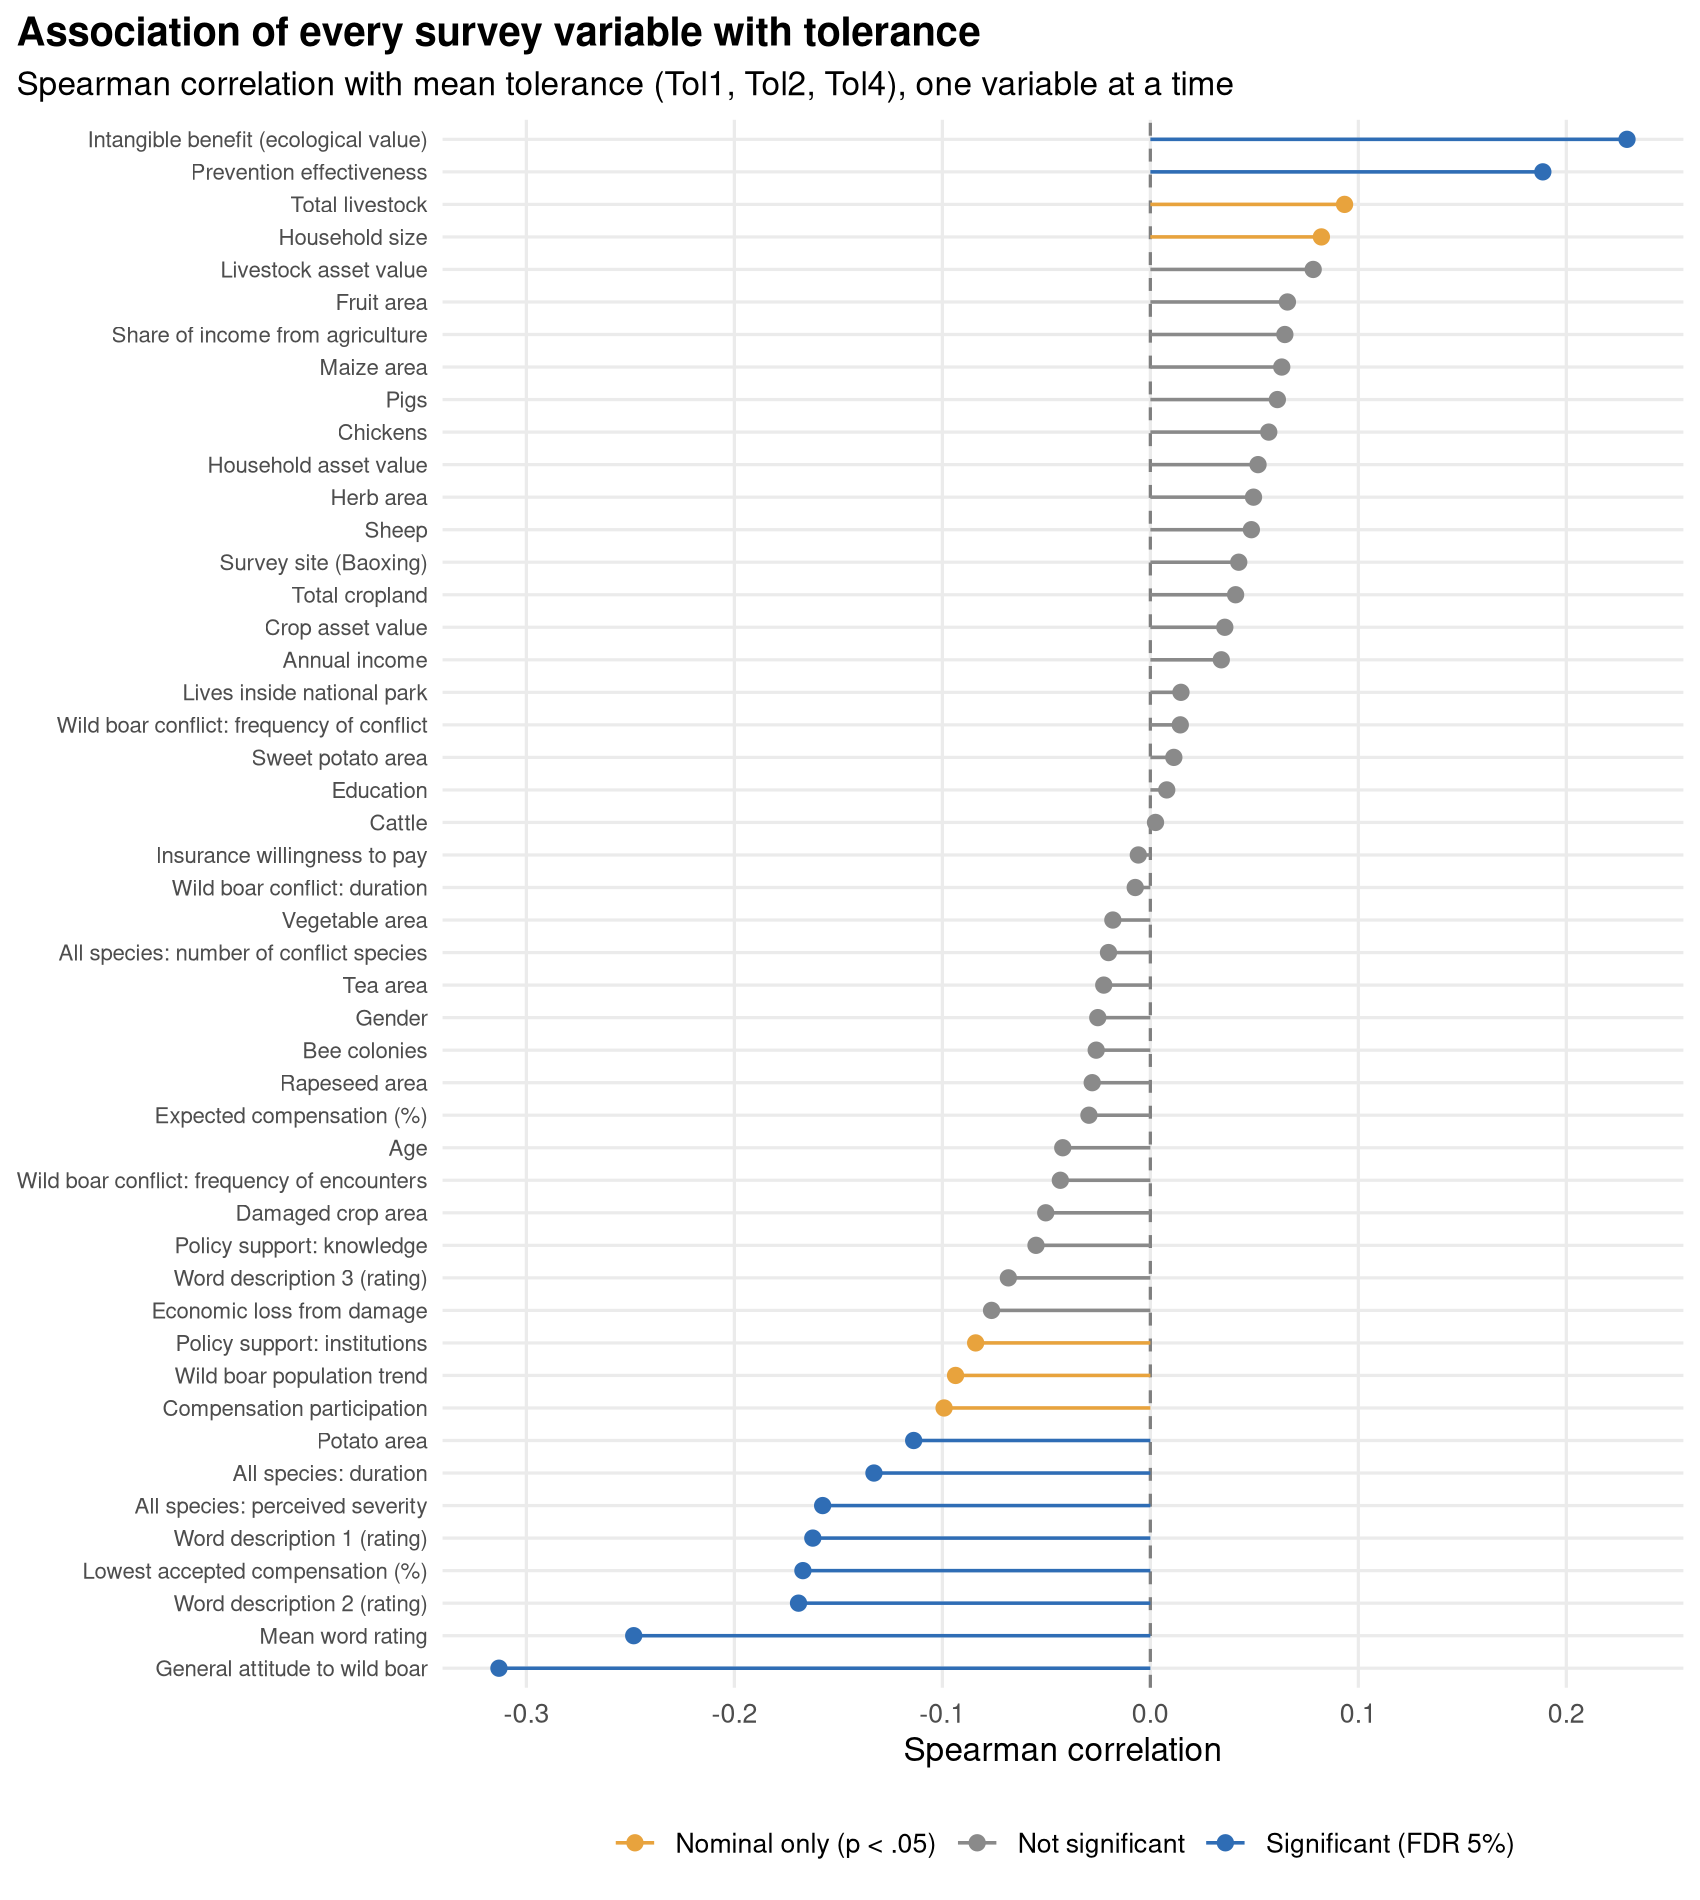
\includegraphics[width=0.9\textwidth]{figures/fig_covariate_screen.png}
\caption{Spearman correlation of each survey variable with mean tolerance.}
\label{fig:screen}
\end{figure}

\subsection{Vibration of effects on observed scores}
\label{app:vibration}

We re-ran the vibration-of-effects exercise \citep{Patel2015} as an independent
check on observed variables: a linear regression of mean tolerance on
compensation participation, with every subset of 13 candidate covariates
(8{,}192 models). The coefficient is negative in all 8{,}192 models and
significant at $p < .05$ in all of them, with a median of $-0.16$ tolerance
points (range $-0.22$ to $-0.09$; Figure~\ref{fig:vibration}). This is a different
estimator from the PLS-based exercise in Section~\ref{robustness:vibration}
(unstandardised coefficient, observed scores), which is why the percentages
differ slightly.

\begin{figure}[htbp]
\centering
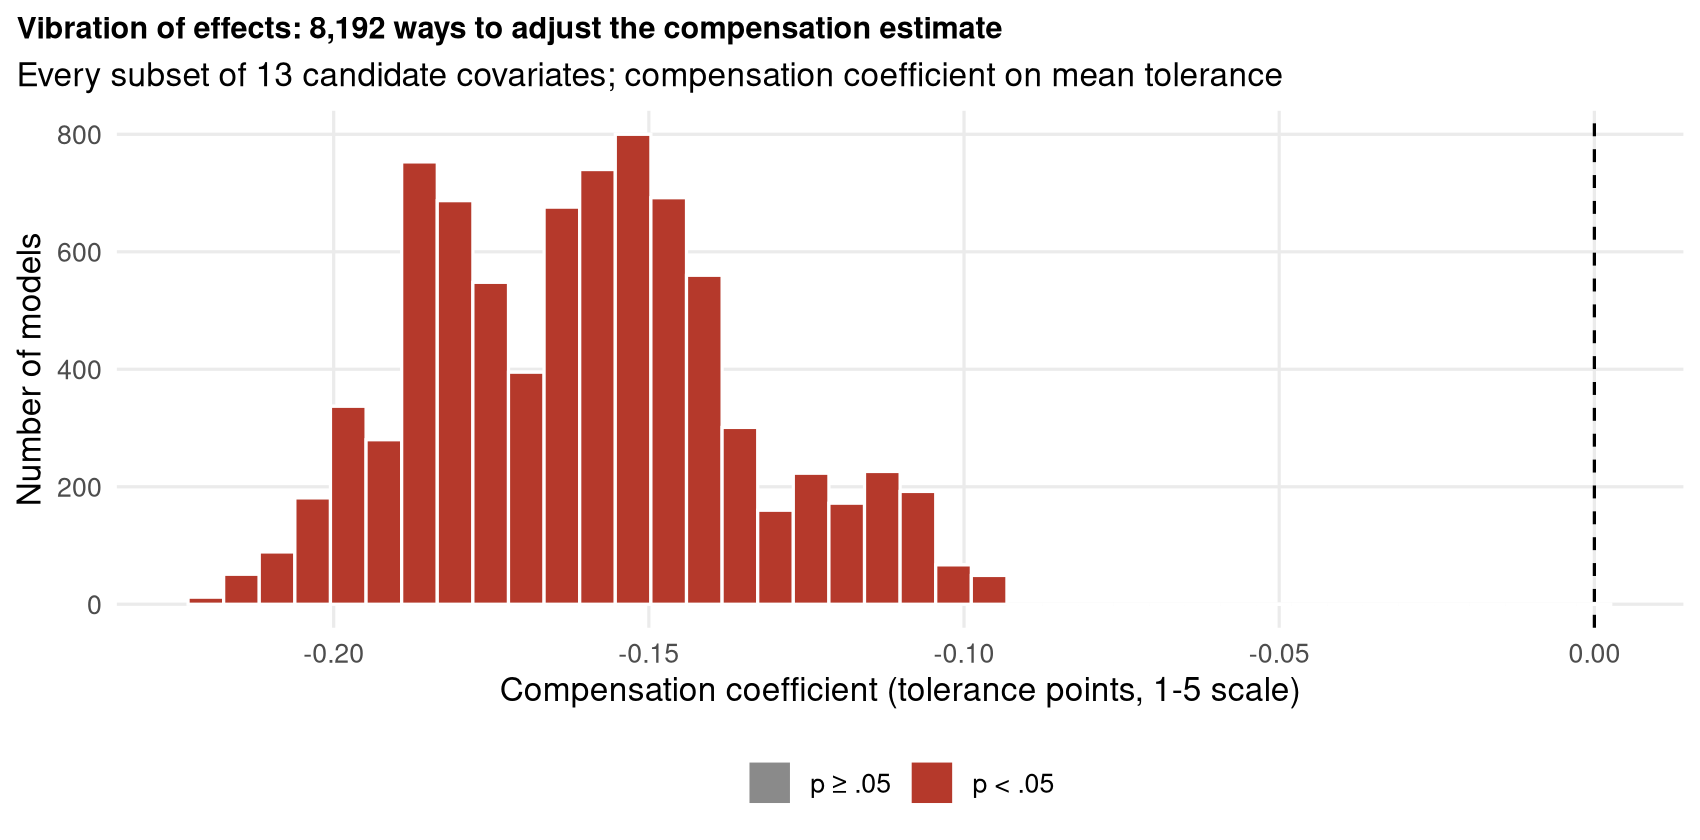
\includegraphics[width=0.9\textwidth]{figures/fig_vibration.png}
\caption{Compensation coefficient across all 8{,}192 covariate subsets.}
\label{fig:vibration}
\end{figure}

\subsection{Effect of the log transformation}
\label{app:transform}

\begin{table}[htbp]
\centering
\caption{Observed-score regression of tolerance on compensation participation
and the same covariates as in Section~\ref{model:rq1}, with the money variables
(income, household assets, economic loss) in four forms. Columns give the
coefficients of compensation participation, intangible cost, and intangible
benefit, and the $p$-value of household assets (robust HC3 standard errors).}
\label{tab:transform}
\small
\begin{tabular}{lrrrrr}
\hline
\textbf{Money variables} & $R^2$ & \textbf{Compens.} & \textbf{Int.\ cost} & \textbf{Int.\ benefit} & $p$ (assets) \\
\hline
$\log(1+x)$ (primary) & .189 & $-0.168$ & $-0.301$ & 0.109 & .026 \\
Raw RMB               & .186 & $-0.165$ & $-0.294$ & 0.109 & .064 \\
Raw, standardised     & .186 & $-0.165$ & $-0.294$ & 0.109 & .064 \\
Rank                  & .187 & $-0.167$ & $-0.303$ & 0.107 & .050 \\
\hline
\end{tabular}
\end{table}

\newpage

\section{Electronic appendix}
\label{el_app}
The electronic supplement accompanying this report contains the following,
organized as a single project repository:

\begin{sloppypar}
\begin{itemize}
  \item \textbf{This report}, as both LaTeX source
    (\url{Schreiben_Wild_boar_compensation_and_tolerance/}) and
    compiled PDF.
  \item \textbf{The presentation slides} delivered on 22 September 2026, as
    PDF (\url{Final_Presentation.pdf}).
  \item \textbf{Analysis code}, organized as a \texttt{targets} reproducible
    pipeline (\url{latest_analysis/scripts/}), with one numbered script
    per analysis stage (data preparation, exploratory data analysis,
    exploratory and confirmatory factor analysis, principal component
    analysis, the primary structural model, mediation, moderation,
    multi-group analysis, robustness specifications, the sensitivity checks
    of Section~\ref{discussion:sensitivity}, and reporting).
    Running the pipeline end to end reproduces every number, table, and
    figure in this report from the raw survey data.
  \item \textbf{Output artefacts}: intermediate and final tables, figures,
    and fitted model objects (\url{latest_analysis/output/}), and a full
    standalone analysis write-up
    (\url{Wildboar_Compensation_Analysis_FULL_offline.html}) covering
    additional diagnostic detail beyond the scope of the main report.
  \item \textbf{The raw and cleaned survey data}, together with the project
    exposé supplied by the project partner
    (\url{docs/Expose_LMU_Compensation_Kou.pdf}), subject to the data
    protection and usage restrictions agreed with the project partner.
\end{itemize}
\end{sloppypar}

Code is documented with in-line comments explaining the purpose of each
script and, where a choice is non-obvious, the reasoning behind it; each
script can be run independently given the cleaned data object it depends on,
and the full pipeline can be run end to end via \texttt{targets::tar\_make()}.
We aspire to, without formally certifying, the standard of the
\emph{Biometrical Journal}'s Checklist for Code Supplements.


\newpage

% ------------------------------------------------------------------------------
% DECLARATION OF AUTHORSHIP-----------------------------------------------------
% ------------------------------------------------------------------------------

\Large
\noindent
\textbf{Declaration of authorship} 
\vspace{0.5cm}
\noindent
\normalsize

I hereby declare that the report submitted is my own unaided work. All direct 
or indirect sources used are acknowledged as references. I am aware that the 
Thesis in digital form can be examined for the use of unauthorized aid and in 
order to determine whether the report as a whole or parts incorporated in it may 
be deemed as plagiarism. For the comparison of my work with existing sources I 
agree that it shall be entered in a database where it shall also remain after 
examination, to enable comparison with future Theses submitted. Further rights 
of reproduction and usage, however, are not granted here. This paper was not 
previously presented to another examination board and has not been published.
\\

\vspace{1cm}
\textcolor{orange}{Location, date} \\

\vspace{3cm}

\noindent\rule{0.5\textwidth}{0.4pt} \\

\textcolor{orange}{Name}

% ------------------------------------------------------------------------------

\end{document}
